\documentclass[]{article}
\usepackage[hidelinks]{hyperref}
\usepackage[pdftex]{graphicx}
\usepackage{float}
\usepackage{subcaption}
\usepackage{wrapfig}
\usepackage[labelformat=empty]{caption}
\usepackage{multicol}
\usepackage{sidecap}
\usepackage{fullpage}
\usepackage{enumitem}
\usepackage{color}
\DeclareMathSizes{10}{10}{10}{10}
\graphicspath{{images/}}

% Color definitions for the legacy and addendum boxes used in the text.
\definecolor{legacy-content}{RGB}{245,250,220}
\definecolor{addendum-content}{RGB}{233,222,219}

% Syntax for intra-document section links.
\newcommand{\jump}[1] {\textbf{``\nameref{sec:#1}}''}

% Syntax for legacy boxes.

\newcommand{\legacy}[1] {
\begin{center}
\colorbox{legacy-content}{
\begin{minipage}[t]{0.95\linewidth}
#1
\end{minipage}
}
\end{center}
}

% Syntax for addendum boxes.

\newcommand{\addendum}[1] {
\begin{center}
\colorbox{addendum-content}{
\begin{minipage}[t]{0.96\linewidth}
#1
\end{minipage}
}
\end{center}
}

% Syntax for bold-faced steps, as used in ``Putting it all Together''.
\newcommand{\step}[1] {
\vspace{12pt}
\noindent \textbf{Step #1}
}

% Syntax for bold-faced listing, similar to the ``Step'' stuff used above.
\newcommand{\boldlist}[1] {
\vspace{12pt}
\noindent \textbf{#1}
}

% Syntax for figures that all full-width, displayed inline.
\newcommand{\fullfigure}[1] {
\begin{figure}[h!]
\includegraphics[width=\linewidth]{#1}
\end{figure}
}

\newcommand{\fullfigurecaption}[1] {
\begin{center}
\vspace{-12pt}
#1
\end{center}
}

\begin{document}
\pagenumbering{gobble}

\title{ \begin{figure}[h!] \centering 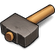
\includegraphics[scale=.8]{logo}
\end{figure}
\textbf{Dwarf Therapist}\\Version 23.2 \emph{Beta} Guide}
\author{Resident Mario}
\date{\today}
\maketitle

\newpage
\pagenumbering{arabic}
\begin{center}
\textbf{Table of Contents}
\end{center}
\tableofcontents
%\vfill
%\begin{figure}[h!]
%\centering
%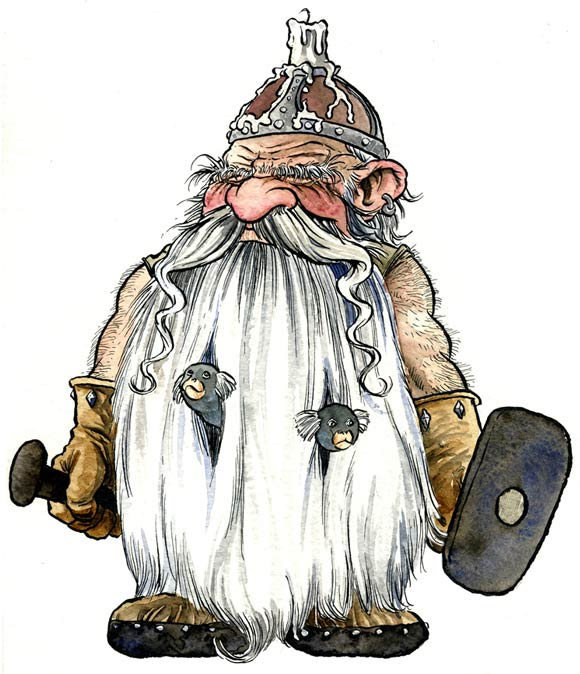
\includegraphics[scale=.35]{Illustration2}
%\end{figure}
%\vfill
\newpage

\part{Preamble}
\section{What's a Dwarf Therapist?}

Dwarf Fortress is not an easy game to play, and many a stoic a gamer has fallen trying to learn how. A
mind-bogglingly complex game wrapped in an extremely simple ASCII\footnote{Technically Code Page 437, an
IBM ASCII expansion sometimes referred to as ``extended ASCII''.} character-based graphics set, Dwarf
Fortress is renowned for being impossible to learn, impossible to play, and impossible to master, and so
caters to a certain, how to say, esoteric crowd.
Luckily the kinds of people that play Dwarf Fortress also happen to be the kinds of people that enjoy
laboring over computer programs that, among other things, aim to make playing the game less of a painful
experience. Dwarf Fortress's community has lovingly crafted countless tilesets, character
mappings, mods, graphical visualizers, companion programs, launchers, debuggers, memory access tools,
plug-ins, extensions, program packages, so on, so forth, you get the idea, to extend and empower this
(projected) 20 year project of a game.

One such gamer is Trey Stout (or chmod, as he's known on the forums) and one such program is Dwarf
Therapist. Initially released in 2009, the program solves one of the most basic and annoying
problems with the game---the difficulty involved in setting Dwarven labor preferences. In the vanilla
game, the only way to set dwarven labor preferences (probably the most important setting there is, dwarf-
wise) was to get to the dwarf, get to their labors screen, and then crawl through a tedious menu bumping
this labor off or this one on.
A starting group of seven dwarves? Not fun, but in grander scheme of the game, doable. 200 of them
running amok? No way. Dwarf Therapist solved this problem  by providing a functional tabular
interface, plugged into the Dwarf Fortress memory, which allows the reading, editing, and committing of
dwarven labor changes.\footnote{Dwarf Therapist was not the first such program of its kind; before it
most players used a similar utility known as Dwarf Manager. But the program became outdated and fell out
of use, and Dwarf Therapist became---and has remained---the de facto standard.}

So, if all it does is manage dwarven labors, what's so difficult about it that it necessitates a
fifty-plus page guide? As it so happens, chmod didn't release the basic version of Dwarf Therapist and
leave it there. He continued working on it, polishing off its interface and new feature. When
he retired from maintaining it in 2010, DwarfEngineer took over its development through 2012; Splinterz
revealed his code fork of the program in February 2013, the currently standard therapy branch. Years of
development have expanded the capacities of the program well past basic labor management and have turned
it into a pretty comprehensive fortress management tool, of which tabular labor management is only the
most obvious and immediately visible application. It's a program that's long since become complicated
enough to necessitate a guide to go with it.

\newpage

\section{Installation}
\label{sec:Installation}
Different distributions of Dwarf Therapist are available for different operating systems. Dwarf Therapist
is a large part of the standard Dwarf Fortress utilities package, so player packs containing the
utility are also widely available.

\vspace{12pt}

\indent\textbf{Windows:} Windows is the development operating system for Dwarf Therapist; a ZIP of the
most recent version can be downloaded directly from the Dwarf Fortress File Depot: 
\url{http://www.bay12forums.com/smf/index.php?topic=126076}. The program will look through your
active programs to try and find the game, so you should generally be safe running it from just about
anywhere, even a thumb drive, but it's most logical to stick it in the Dwarf Fortress root
directory---the one with the game's .exe file.

As of \today, the standard Windows bundle for the game containing Dwarf Therapist is the Dwarf Fortress
Starter Pack: \url{http://www.bay12forums.com/smf/index.php?topic=126076}.

\vspace{12pt}

\textbf{OSX:}
Dwarf Therapist has been ported to Mac, and is available here:
\url{http://dffd.wimbli.com/file.php?id=9127}.

The current standard starter pack for Mac is the MacNewbie Pack, available from here:
\url{http://dffd.wimbli.com/file.php?id=7922}.
\vspace{12pt}

\textbf{Linux:}
There is no standard Linux release. You can also build it yourself from the source with the instructions
available here: \url{http://code.google.com/p/dwarftherapist/wiki/BuildingDwarfTherapist}.

\section{About this Guide}
\label{sec:About this Guide}

The bulk of this guide was written by Resident Mario over the course of a few weeks in the summer of
2013, as a \LaTeX \space exercise. In the summer of 2014 he made the document's source code public,
with the hope is that in the future this guide will be maintained by the community, rather than any one
busy and fallible author.

Splinterz has continued active development on the utility, and additionally the summer of 2014 saw the
release of the next major version of Dwarf Fortress, two years in the works, version 0.40. As such, the
version of Dwarf Therapist that you see now has been refined quite a bit over the one that was originally
covered by this guide. Dwarf Therapist's capacities were exploited over the course of the writing of this
guide in program-solving exercises, some of which, particularly in terms of the program's look and feel,
have since been ``solved'' (often by the inclusion of features that the author themselves recommended).
Some other usecases have since been included in the program's base installation. In order to
maintain this guide's overall narrative format, for the most part the usecases used now are the same
ones used when this guide was first written, even in cases where they may seem redundant or have since
been hard-coded into the utility---just because the changes are no longer novel, doesn't mean that they
aren't still useful exercises. Usually, a inset ``legacy box'' is provided to inform the reader that the
default behavior has since changed, and to describe the way things ``used to be''.

Additionally, because Dwarf Therapist and Dwarf Fortress have been updated several times, in the latter
case in ways that break compatibility with old saves, example illustrations may use old views until a new
fortress can be played sufficiently in new release versions to generate the needed usecases.

\newpage

\part{Basics}
\section{Connecting to Dwarf Fortress}
\label{sec:Connecting to Dwarf Fortress}

Dwarf Therapist requires Dwarf Fortress to be running and an active fortress to be open within the game
in order to work properly. You can open the utility without the game running or without a fortress
loaded, but it will complain to you:

\begin{figure}[h!] \centering
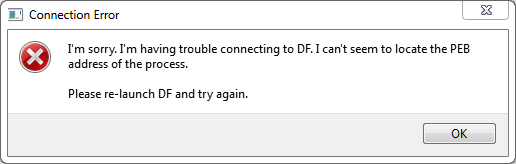
\includegraphics[width=.7\linewidth]{Sec1Fig1}
\end{figure}

This is because before Dwarf Therapist can do much of anything useful, it has to connect to a running
instance of the game; the only function that the utility can provide by itself is the ability to write
filter scripts (which obviously can't be applied out-of-game), move the docks around, and change some
settings. You'll get another, similar error message if you load a fortress, connect to the game, and then
unload it:\footnote{This behavior can be disabled in the general options. However, this is no ``offline''
mode: cycling out of a fortress, making changes, loading it again, and then attempting to commit your
offline changes will only cause the utility to crash.}

\begin{figure}[h!] \centering
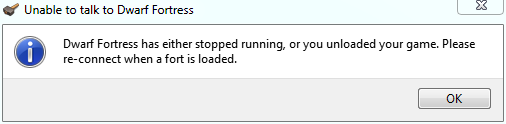
\includegraphics[width=.7\linewidth]{Sec1Fig2}
\end{figure}

\begin{wrapfigure}{R}{0.35\textwidth}
\vspace{-20pt}
  \begin{center}
    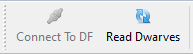
\includegraphics[scale=1]{Sec1Fig3}
  \end{center}
  \vspace{-10pt}
  \end{wrapfigure}
  
To avoid such messages you should generally launch Dwarf Therapist second and close it first, but it
doesn't really matter too much---you can connect at any time using the ``Connect to DF'' button on the
main toolbar. To keep its memory usage down, Dwarf Therapist connects to your game intermittently, loading
data into the utility only when a fortress is first opened or when you request to do so. This is the
function of the second button on the main toolbar, ``Read Dwarves'', which will easily be the most used
item on your main toolbar.\footnote{Since Dwarf Therapist now lets you view animals, too, the name is a
bit of an anachronism. If you mod your game and change the playable race, the button label will actually
change with it---one of Dwarf Therapist's many mod-friendly features.} Loading data into the game only
takes a fraction of a second to a few seconds (depending on the size of your fortress) each time, and it
can be done regardless of whether the game is paused or not---but since you're probably going to be
spending some time on the Therapist screen once you switch to it, pausing is probably a good idea.
\newpage

\section{Main Display}
\label{sec:Main Display}
Once you've connected to and loaded a fresh fortress into Dwarf Therapist, your screen should look
something like this:

\fullfigure{Sec1Fig4}

\subsection{Labors View}
\label{sec:Labors View}
\fullfigure{Sec1Fig5}

Most of the screen space is taken up by the the graphical management user interface
(or \emph{view}), the main window visible onscreen. Since we've only just created our fortress it doesn't
have many members yet, and so most of the view is whitespace.

The labors view visible here is the most important and immediately accessible part of the program,
and is the feature around which the rest of Dwarf Therapist is built. Toggling labor preferences has
been the primary purpose of Dwarf Therapist from its very first release, and many users still use it for
little else; but Dwarf Therapist has since become an expansive management utility with an
extensive suite of tools and capacities that this guide will attempt to illuminate in greater depth.

It should be noted that there are more labor preferences available in the game
then can be comfortably and compactly fit into the screen, necessitating that we contend with a scroll
bar at the bottom of the screen on all but the widest of monitors; a second one appears on the right once
your dwarves get too numerous (vertically) to fit into the interface.\footnote{For tips on
formatting your display for compactness, see the section \jump{Formatting Your Display}.}

Labors are organized into ``tranches'', with related labors categorized and sorted under industry
allegiances roughly like the color assignments used by dwarves of those professions in-game:
\fullfigure{Sec1Fig6+}

These labors should be familiar to players of the game, as should be their categorical
professions: miners, woodworkers, stoneworkers, rangers, doctors, farmers, fishery workers, metalsmiths,
jewelers, craftsdwarves, engineers, and peasants.

\legacy{

In older versions of Dwarf Therapist, the default view sorted labors in the exact
same order and with the exact same colors that Dwarf Fortress sorts them:

\vspace{12pt}
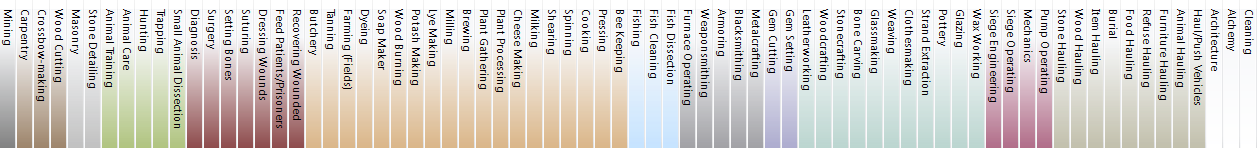
\includegraphics[width=\linewidth]{Sec1Fig6}
\vspace{2pt}

The view is still available in the view add dropdown menu as the ``Labors Alt'' view. It has been
replaced as the default by the more polished ``Labors'' view, written over the course of this guide
(see \jump{Custom Grid Views}) and then introduced into Dwarf Therapist as the new default shortly
thereafter.

}

To the left of the labor columns are dwarfwise informational columns: a gendered list of your dwarves,
alphabetically ordered, flanked by a color gradient for their equipment status, icons representing their
(current) job, a color gradient their happiness, and another set of icons their profession. Since we
jumped into this view immediately after our fortress disembarked, our dwarves have neither jobs nor
variance in their happiness just yet, but they do exhibit the different professions I've selected for my
starting set. Dwarves which reach legendary status in at least one skill will have their names displayed
in boldface. to distinguish them from their ``lesser'' brethren.

Clicking on a headers at the top of the screen for any of the columns allows us to sort the list by that
column; click on it again to reverse the sort order, or on another column to go to that sort instead.
The name spacer lists your dwarves alphabetically, the job header sorts them by Job ID, happiness by
happiness level, and equipment by whether or not they are fully clothed and,
if their job requires a tool, have that tool at hand.\footnote{\label{footnote} Job IDs and
the related Profession IDs are somewhat abstract lists of jobs and professions, respectively, whose
modification we will discuss much later in this guide. For further reference, see \jump{Profession IDs}
in the appendix.} Hitting the actual labor columns will sort your dwarves in two tiers, first dwarves
with that labor enabled by their experience level, then dwarves without it enabled by the same
metric.\footnote{Dwarves accumulate experience levels and ``rank up'' their skill level every time they
pass a certain milestone.} If \emph{none} of your dwarves have experience in a task, sorting won't
actually do anything.

Within the grid itself the numbers demarkate the skill level of the dwarf at a task while the shading
tells you whether or not they have it enabled. Try clicking on a few of the cells and seeing how the
program responds---getting labor changes into the game should be entirely intuitive, even if we're not
going over it in detail just yet.

% \begin{wrapfigure}{R}{0.32\textwidth}
% \vspace{-20pt}
%   \begin{center}
%     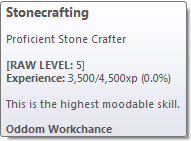
\includegraphics{Sec1Fig7}
%   \end{center}
% \vspace{-10pt}
%   \caption{The labor tooltip.}
% \end{wrapfigure}
\newpage

\begin{wrapfigure}{R}{0.55\linewidth}
\vspace{-10pt}
  \begin{center}
    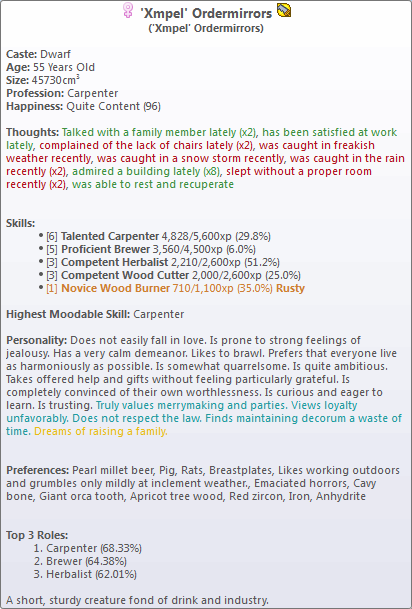
\includegraphics[scale=.8]{Sec1Fig8}
  \end{center}
\end{wrapfigure}

One major feature of the grid interface is its tooltips, which pop up whenever you hover over a space in
the grid. Hovering over the labor column headers will tell you how many dwarves have that labor enabled,
while hovering over individual labor cells will display the descriptive (Dabbling, Novice, Adequate,
Competent, etc.) and raw (0, 1, 2, 3, etc.) skill that dwarf has in that labor, their cumulative
experience and progress towards the next skill level, whether or not that is their highest moodable
skill, and (if they are legendary from a strange mood) the name of the artifact they crafted; if the
skill has rusted, that information will appear here as well.\footnote{
\href{http://dwarffortresswiki.org/index.php/DF2012:Skill\#Skill_rust}{\textbf{Skill rust}} occurs when
a dwarf has not performed the labor associated with a skill for a long time. Dwarves whose skills are
``Very Rusty'' will eventually see their skill in the labor drain away or even vanish completely.}
Hovering over a dwarf's happiness gives you a dwarf's exact happiness score, hovering over their current
job gives the numerical ID of that task, and hovering over their equipment gives you their current
clothing and tools carried.

By far the most information-dense tooltip on display is that of the dwarves themselves. Hovering over a
dwarf's name will give you their caste,
\footnote{\href{http://dwarffortresswiki.org/index.php/DF2012:Caste}{\textbf{Castes}} are raw file
definitions used to define species or sub-species, and are not very useful in vanilla Dwarf Fortress:
but having a display for them is handy if you're using mods and have fiddled with your playable race.}
gender, profession, happiness level, thoughts (color coded green when good, red when bad), skills (rust
will be highlighted), personality, preferences, and their calculated ``Top 3 Roles'' (covered later, see
\jump{Roles}). The dwarven caste description, more or less memorized by the community, also makes an
appearance, at the end of the tooltip. The information to be displayed here can be included or excluded
as you please by adjusting the appropriate settings in \texttt{Options > Tooltip}.

\newpage

\subsection{Views}
\label{sec:Screens Tab}
Immediately above the labors screen is the screens tab:

\begin{figure}[h!]
\centering

\includegraphics{Sec1Fig9}
\end{figure}

Although the Labors view is the core of the interface, and is the tab open by default, there's a number
of other screens built into the utility, all of which are available for your use. The screens tab has
several of these tabs open by default, and more are available under the ``Add'' menu in alphabetical order.
The tabs can be moved around, deleted, and re-added as much as you want, and the utility will save their
state between instances, allowing you to keep your favorite tabs around where you'd like them. You can
also have multiple instances of a tab open---although this isn't a particularly useful feature, it's
there. A list of the screens and what they do follows:

\begin{wrapfigure}{L}{0.35\textwidth}
\vspace{-10pt}
  \begin{center}
    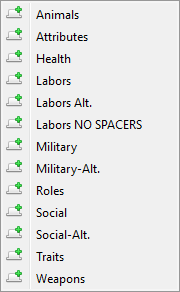
\includegraphics{Sec1Fig10}
  \end{center}
\vspace{-70pt}
\end{wrapfigure}
\noindent\textbf{Animals:} Lists domestic, caged, and tame creatures and their attributes. Includes
whether or not they are marked for butchering and whether or not they are caged. Distinguishes between
children and adults, and lists current training levels. This view is unique in that it is the only one
not directed at your dwarves.


\boldlist{Attributes} A basic list of attributes. Tranches are physical, then mental.


\boldlist{Health} A detailed breakdown of all of your dwarves' wounds and ailments.


\boldlist{Labors} A compressed alternative to the legacy Labors view that was originally created
as part of this guide, and has since been packaged into the utility as the new default: see the section
\jump{Creating Your Own Grid Views}.


\boldlist{Labors Alt} The Labors View is the program's legacy primary view---for a detailed
description see \jump{Labors View}.


\boldlist{Labors NO SPACERS} Same as the Labors view, but without any spacers between the
categorial professions, winning back some screen space.


\boldlist{Military} Allows you to view your dwarves' combat ability. It lists the relevant combat
skills in melee, fighter, equipment, miscellaneous, and marksdwarf tranches, then gives you a view of
their combat-related attributes,  then their compatibility scores for various combat roles, then which
weapons they are or are not able to equip based on their relative size.\footnote{Theoretically all the
but the runtiest of dwarves are able to wield all but a few especially large non-native weapons
one-handed; however, because of a bug, in Fortress Mode \emph{no} dwarves can wield two-handed weapons,
ever.}


\boldlist{Military-Alt} Expands on the regular Military view by including role ratings.


\boldlist{Roles} Lists the role ratings of your dwarves, a score out of 100 that tells you how
adapted they are to that profession. This view is discussed in \jump{Using Roles---The View Method}.


\boldlist{Social} Catalogues your dwarves' social skills. The tooltip lists related
roles, which are only present for some of the social skills.


\boldlist{Social-Alt} Expands on the regular Social view by including role ratings, as well as a
non-social trait columns for traits are affected by social traits. For example, Assertiveness is added
and grouped with Persuader, because having low assertiveness means it's impossible to increase the
persuader trait.


\boldlist{Traits} This is a special view that lists raw role ratings; see above.


\boldlist{Weapons} Lists dwarves by which weapons they can wield. This view is
dynamically generated: in vanilla it acts as a subview of the military view, but mods with large amounts
of weapons will look significantly more expansive. Additionally, the weapons view will be tacked on to the
military view as well if there are ten or fewer weapon groups.

\subsection{Group By and Filters}
\label{sec:Group By and Filters}
\begin{figure}[h!]
\centering

\includegraphics[width=\linewidth]{Sec1Fig11}
%
\includegraphics[scale=.78]{Sec1Fig11}
\end{figure}

Filter scripts are an advanced topic covered in \jump{Filter Scripts}, and will not
be covered in depth here. For now, know that the ``Filter Dwarves'' input field is the quickest way to find individual dwarves by name.

The Group By menu, meanwhile, changes what your dwarves are sorted by in the views, and is fairly
intuitive, mostly useful for examining various demographic breakdowns of your fortress. Options are:
\vspace{12pt}

\begin{wrapfigure}{R}{0.225\textwidth}
\begin{center}
\vspace{-10pt}
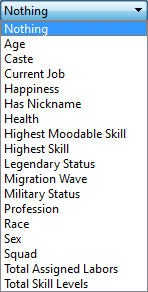
\includegraphics[scale=.85]{Sec1Fig11+.png}
\vspace{-20pt}
\end{center}
\end{wrapfigure}
\noindent Nothing, the default.

\noindent Age, in tiers of ten.

\noindent Caste, all dwarves in vanilla outside of the Animals view.\footnote{When mods are active an
additional ``Caste Tag'' option becomes available, useful for finding hidden or secret castes that may
exist.}

\noindent Current Job, a breakdown of the stuff your dwarves are doing.

\noindent Happiness, the sort does a better job.

\noindent Has Nickname, yes or no, useful when you're naming dwarves.

\noindent Health, health status.

\noindent Highest Skill, a demographic sort.

\noindent Highest Moodable Skill, useful when grinding for a legendary armorsmith.

\noindent Legendary Status, yes or no.

\noindent Migration Wave, the utility's best historical sort, and therefore
a go-to grouping.

\noindent Military Status, active, off duty, can activate, or noble.

\noindent Profession, perhaps less useful than the equivalent sort.

\noindent Race.\footnote{A creature's race is
defined off of its raw file, and will be the same as its caste in most cases. The exception is when a
sub-special caste exists---in which case, race and caste does in fact diverge.}

\noindent Sex.

\noindent Squad, No Squad or 
*Squad Name*.

\noindent Total Assigned Labors, a numerical statistic.

\noindent Total Skill Level, another numerical statistic.
\vspace{12pt}

When a group is active it will be expandable and collapsible, and in the collapsed labors view will
display the lowest happiness of the group as well as (for each skill) if anyone in the group has the
skill enabled, resulting in a darkened box with a numerical dwarf count or, if they all have it enabled,
in a green box. This feature can be toggled on or off in the options. Groups consisting entirely of
children will appear bright green. For more on using groups, see \jump{Using Groups}.

\newpage
\subsection{Population Indicator and Status Bar}
\begin{wrapfigure}{R}{0.40\textwidth}
\vspace{-20pt}
  \begin{center}
    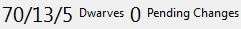
\includegraphics[width=0.38\textwidth]{Sec1Fig12}
  \end{center}
\vspace{-20pt}
\end{wrapfigure}

The population indicator in the top-right corner of the window gives an at-a-glance view of how many
dwarves there are in your fortress, distributed adults/children/babies, and the number of currently
active pending changes (refer to \jump{Managing Your Dwarves}). This lets you keep track of the number of
changes you have pending, though not their nature, without having to pull out the ``Pending Changes''
dock (see \jump{Docks}).

The basic status bar at the bottom of the window provides row and column information on the left, and a
dwarf selection count and Dwarf Fortress version type information on the right.

\vfill

\subsection{Main Toolbar}
\label{sec:Main Toolbar}
\fullfigure{Sec1Fig13}

The main toolbar presents the most important ``shortcuts'' the program has to offer. Except for the
Optimizer, all of the toolbar items have an associated hotkey. Right clicking on the main toolbar allows
you to toggle it (and docks, covered in the next section) on and off, and it can also be accessed under
the ``Window'' menu in the main menu.

\parbox[]{1\textwidth}{}
\begin{itemize}
\item \textbf{Connect to DF}: If Dwarf Therapist is not already connected to Dwarf Fortress, this will
attempt to connect the program. If it is, this will be grayed out. Shortcut \texttt{Ctrl + C}.
\item \textbf{Read Dwarves}: Reads the current state of the dwarves in your fort into the Therapist.
Shortcut \texttt{Ctrl + R}.
\item \textbf{Expand All}: Expands all group views; if Group By is set to ``Nothing'' this will have no
effect. Shortcut \texttt{CTRL + >}.
\item \textbf{Collapse All}: Collapses all group views, doing the opposite of the above command. Shortcut
\texttt{CTRL + <}.
\item \textbf{Clear}: Clears all labor preference changes (see \jump{Managing Your
Dwarves}). Shortcut \texttt{Ctrl + E}.
\item \textbf{Commit}: Commits labor preference changes (see above). Shortcut \texttt{Ctrl + T}.
\item \textbf{Optimize}: Runs an optimization plan. Optimization is an
advanced topic covered in \jump{Optimization Plans}, and this option does not appear on the toolbar at
all if you have no optimization plans defined.
\item \textbf{Options}: Allows you to adjust settings. Will be covered in the section
\jump{Options}.
\item \textbf{Exit}: Exits the application.

\end{itemize}

\vfill
\newpage
\subsection{Docks}
\label{sec:Docks}
%\begin{wrapfigure}{R}{0.33\textwidth}
%\vspace{-20pt}
%  \begin{center}
%    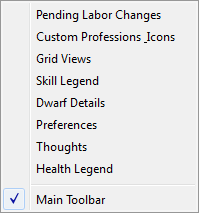
\includegraphics[width=0.33\textwidth]{Sec1Fig15}
%  \end{center}
%\vspace{-10pt}
%\end{wrapfigure}

When you first open Dwarf Therapist, the right side of the screen will host a couple of docks. These two
marvelous boxes are used to keep pace with what you're doing and modify how Dwarf Therapist works in
various ways. Up to a trio of docks can be attached to the right side of the screen, and others can be
pinned against other cardinal directions (or simply left floating around). Clicking the window button
detaches the dock and leaves it to float, while clicking on the X button closes them, giving the others
more room. If you don't have any docks at all pinned to a the right side, the main view will expand to
make use of the new screen space.

By grabbing and dragging a dock you can actually attach anywhere on the screen---to the left, above,
below, or to the right of the main view. By grabbing and dragging it into another dock, you can tab them,
so that the dock that is currently open gets to monopolize the screen space. And the current dock
configuration is saved between instances of the program, of course. Note that the main menu is actually
also a dock, albeit one that must stay independent when docked, and so can be moved anywhere or even
gotten rid of entirely. A list of docks follows:

\boldlist{Dwarf Details} This one lists a lot of stuff, so if you use it you should tab-dock
it. Dwarf Details provides an expanded view of a dwarf's abilities, providing pretty much all of the
information on their capacities in the various views (and then some) in one comprehensive tabular form.
You've got name, translated name, age, profession, current job,  happiness level, skills table with
progress bars, attribute table with maximum trainable value and message text, raw trait value with
message text, top ten role ratings, and a table of the dwarf's preferences.

\begin{figure}[h!]
        \centering
        \begin{subfigure}[C]{0.45\linewidth}
                \centering
                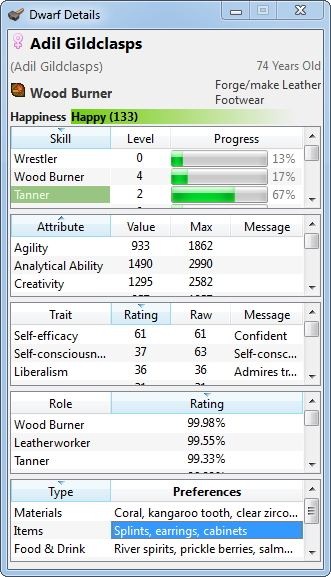
\includegraphics[width=.75\textwidth]{Sec1Fig16-1}
        \end{subfigure}~
        \begin{subfigure}[C]{0.45\linewidth}
                \centering
                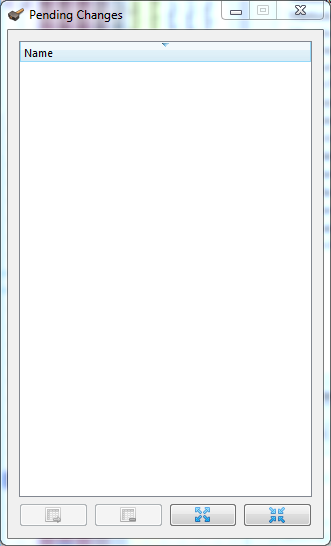
\includegraphics[width=.8\textwidth]{Sec1Fig16-2}
        \end{subfigure}
\end{figure}


\boldlist{Pending Changes} This dock displays which labors you are turning on or off in a
tabular form, and allows you to commit or clear your changes independent of the main toolbar.
Originally called ``Pending Labor Changes'', the dock has been renamed in lieu of the fact that it now
also displays, and allows the manipulation of, nickname, profession, and squad assignments, all things
we'll discuss in time. There are also buttons for expanding and collapsing changes displayed in the dock,
useful when making mass labor swaps. For a discussion on the basics of dwarven management (getting
there!) see \jump{Managing Your Dwarves}.

\boldlist{Customizations} This dock allows you to create, edit, and manage custom professions,
custom icons, and super-labors, all things we'll discuss later in this guide. For a discussion on
creating custom professions, the first of the trio we'll cover, see \jump{Creating Custom Professions}.

\boldlist{Grid Views} Allows you to open grids from a menu, or create entirely new ones of your own
design. See \jump{Creating Your Own Grid Views} for more.

\boldlist{Skill Legend} Provides a legend for skills display onscreen, and allows you to quickly
change it with a drop-down menu. Only really there for completeness.

\boldlist{Preferences}: Lists your dwarves by preferences, and allows you to search through them by
object of preference. Clicking on one or more of the preferences allows you to filter dwarves so that
only those with that preference are displayed on-screen (and Clear Filter obviously clear the filter).

\boldlist{Thoughts} Similar to the Preferences dock, this brings up popular thoughts by count,
allows you to search through them, and allows you to filter your dwarves by them.

\begin{figure}[h!]
        \centering
        \begin{subfigure}[C]{0.5\linewidth}
                \centering
                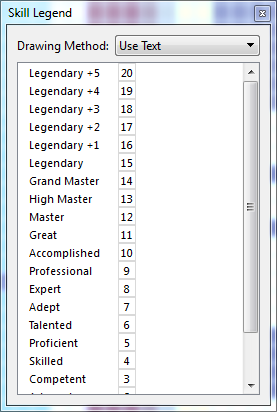
\includegraphics[width=.75\textwidth]{Sec1Fig16-4}
        \end{subfigure}
        \begin{subfigure}[C]{0.45\linewidth}
                \centering
                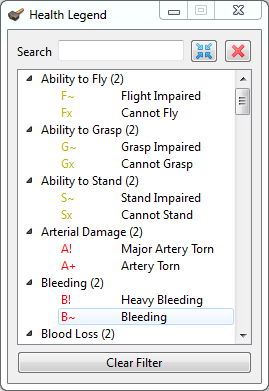
\includegraphics[width=.8\textwidth]{Sec1Fig16-3}
        \end{subfigure}
\end{figure}

\boldlist{Health Legend} The health legend allows you to filter your dwarves by health status, using
the information provided in-game by the health screen. The dock includes mundane irregularities such as
hunger and thirst as well as rather severe conditions like missing limbs and paralysis. This information
is summarized in the Health view.

\newpage
\subsection{Menu Bar}
\label{sec:Menu Bar}
\fullfigure{Sec1Fig17}

The last piece of Dwarf Therapist we're going to analyze is the iconic menu bar (or taskbar), present on
almost every real application ever written. I'm going to give a brief list of what's in it here, and
direct you to the sections for specific functions when appropriate.

\vspace{12pt}
\begin{wrapfigure}{R}{0.40\textwidth}
  \begin{center}
    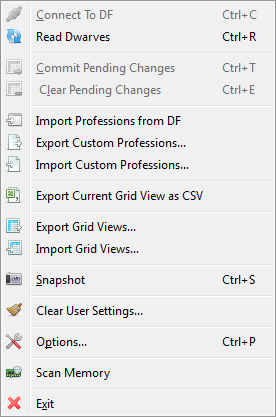
\includegraphics[width=\linewidth]{Sec1Fig18}
  \end{center}
\vspace{-120pt}
\end{wrapfigure}

\boldlist{\indent File} provides a smorgasbord of options:

\boldlist {Connect to DF} \texttt{(CTRL + C)} See \jump{Connecting to Dwarf
Fortress}.

\boldlist {Read Dwarves} \texttt{(CTRL + R)} See link above.


\boldlist {Commit} \texttt{(CTRL + T)} See \jump{Managing Your Dwarves}.


\boldlist {Clear} \texttt{(CTRL + E)} See link above.


\boldlist {Import Professions from DF} See \jump{Exporting and Importing Professions}.


\boldlist {Export Custom Professions} See link above.


\boldlist {Import Saved Custom Professions} See link above.


\boldlist {Export Current Grid View as CSV} Exports the current view as a ``comma exported value''
spreadsheet, which is a basic \texttt{TXT} that can be read by almost any spreadsheet software.


\boldlist {Export Grid Views} Exports, in Dwarf Therapist's \texttt{DTG} export format, a chosen
selection of grid views to a chosen file location.
See \jump{Exporting and Importing Grid Views}.

\boldlist{Import Grid Views} Imports \texttt{DTG} grid views from the disk.
\jump{Exporting and Importing Grid Views}.

\boldlist {Snapshot} \texttt{(CTRL + S)} Takes a snapshot of the currently active Dwarf Therapist
window, and stows it away where you tell it. Basically an extended version of the \texttt{PRNT SCR}
key.\footnote{ This option is functionally limited to full-window shots, and so should not be used too
extensively---the screenshots for this guide, for instance, were done with Greenshot.}

\boldlist {Clear User Settings} Deletes all user settings and then exits Dwarf Therapist. This restores
all settings in the program back to default and erases all data, which is why it has a warning screen---it
can be very damaging if you have complex scripts and other goodies programmed into the utility.


\boldlist {Options} \texttt{(CTRL + P)} Also provided on the Main Toolbar; see \jump{Options}.


\boldlist {Scan Memory} See \jump{Scanning Memory}.


\boldlist {Exit} Immediately exits the program.

\boldlist{\indent Scripting} provides facilities for generating Filter Scripts to apply to your
dwarves. For a detailed discussion on Filter Scripts, see \jump{Filter Scripts}.

\boldlist{\indent Roles} provides facilities for creating, modifying, removing, importing, and
exporting custom roles. For a detailed discussion on Roles, see \jump{Roles}.

\boldlist{\indent Optimizer} allows the creation, modification, deletion, importation, and exportation of
Optimization Plans. For details, see \jump{Optimization Plans}.

\boldlist{\indent Windows} allows you to modify the docks and main toolbar displays in a
manner similar to right clicking on the main toolbar. For more information on Docks, see
\jump{Docks}.

\boldlist{\indent Help} provides links to a few different helpful resources:

\boldlist {Project Homepage} Provides you with a link to the project homepage:\\
\url{https://github.com/splintermind/Dwarf-Therapist}.

\boldlist {Discussion Forums} Provides a link to the master Dwarf Therapist forum thread:\\
\url{http://www.bay12forums.com/smf/index.php?topic=122968.0}.

\boldlist {Request Feature / Report Bug} Provides a link to the Dwarf Therapist issue tracker:
\url{http://www.code.google.com/p/dwarftherapist/issues/entry/}.

\boldlist {Donate} For buying the poor developer a beer through PayPal.

\boldlist {About} Brings up a small splash screen giving you the Dwarf Therapist version number, some
accreditation links, and a link to check for updates.

\newpage
\section{Managing Your Dwarves}
\label{sec:Managing Your Dwarves}
\begin{wrapfigure}{R}{0.20\textwidth}
\vspace{-20pt}
  \begin{center}
    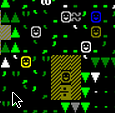
\includegraphics[width=0.20\textwidth]{Sec2Fig1}
  \end{center}
\vspace{-10pt}
\caption{Dwarves frolic by the caravan.}
\end{wrapfigure}
Now that we've finally pinned down all the wayward bits of Dwarf Therapist and explained, though in
some advanced cases quite briefly, what each of them does, we are in a position to discuss the
game's primary source of utility: its ability to change the game's dwarven labor preferences,
without having to deal with the game's clunky dwarfwise interface. This section will cover the basic
tenets of dwarven management and demonstrate why even when Dwarf Fortress updates that have
been in the works for a year or more are released, many people still refuse to play until Dwarf
Therapist is updated to match. If you've already gotten dwarven labor management down pat, you can
skip ahead to \jump{Options}, or to \jump{Advanced Features} if
you're itching to try out the program's more advanced features.

\vfill
\subsection{Making Labor Changes}
\label{sec:Making Labor Changes}
\begin{wrapfigure}{L}{0.025\textwidth}
\vspace{-22pt}
  \begin{center}
    
\includegraphics[width=0.023\textwidth]{Sec2Fig2-1}
  \end{center}
\vspace{-10pt}
\end{wrapfigure}
Now let's return to the seven humble dwarves we touched upon at the beginning of this guide, illustrated
above. We've got two miners, a carpenter/woodcutter, a mason, a stonecrafter/broker, and two farmers. The
woodworker is soon to be off cutting wood, and the two miners are soon to be off digging---but what
should the other four dwarves do? The facilities for their professions haven't been built, and there's
nothing to haul around yet. This is a recurring problem, but I look around and see that there are plenty
of bushes lying around that can be stripped for some free early food (and seeds for an above-ground farm,
later on). So I designate some plants for gathering, and then change the labors to get my dwarves to do
some work for me.

Individually designating dwarven labors for changes is as simple as clicking on the boxes that correspond
with that dwarf and that task in the labor view. The box with either fill or unfill and will be
surrounded by a bright red border, and the exact nature of the labor changes will be added to the pending
labor changes dock if one is present on your screen and notched onto the Pending Changes counter near the
top right of your screen; the Clear and Commit buttons on the main toolbar will greenlight as well. The
changes that we would like to make and how they appear on-screen are highlighted on the left. To revert a
change you're making---if, for instance, you accidentally toggle Plant Gathering on for your Carpenter,
when what you really want him to be doing is chopping trees---just click on it again to revert it to the
previous state.

We've made some labor preference changes, but right now they're only hanging around in the "Pending
Labors" queue in Dwarf Therapist. To make them actually appear in the game, we have to \textbf{commit}
these changes. Here's what the changes we want to make look like in the Pending Labor Changes dock,
expanded for clarity and collapsed for compactness (which is what the buttons do, if you didn't know
already):
\vfill
\begin{figure}[h!]
\vspace{-5pt}
        \centering
        \begin{subfigure}[H!]{0.48\textwidth}
                \centering
                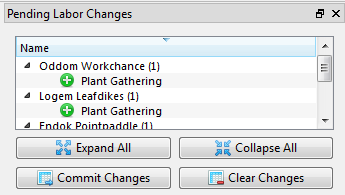
\includegraphics[width=\textwidth]{Sec2Fig3-1}
        \end{subfigure}~
        \begin{subfigure}[H!]{0.48\textwidth}
                \centering
                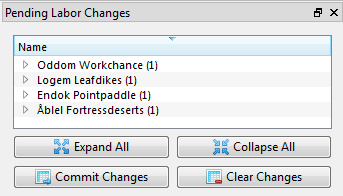
\includegraphics[width=\textwidth]{Sec2Fig3-2}
        \end{subfigure}
\vspace{-5pt}
\end{figure}
You can remove the need for collapsing changes by giving the dock a bit more breathing room.
\vfill

\newpage
\noindent Hitting ``Clear Changes'' will clear all of these changes and wipe Dwarf Therapist to its
previous state, while hitting ``Commit Changes'' will send the new labor orders through to the game,
updating Dwarf Therapist to reflect the changes and producing immediate results. These buttons are
available on both the Pending Labor Changes dock and on the Main Toolbar, however they also have
hotkeys:
\texttt{Ctrl + E} and \texttt{Ctrl + T}, respectively. Since these are two of the most common operations
you'll be conducting with the program, it's probably a good idea to remember these hotkeys---it will save
you a lot of time (refer to \jump{Hotkeys} for the list of available hotkeys).

Dwarves start off with certain labors enabled: labors they have above-dabbling level skill in, hauling
labors (including the two medical ones), and cleaning are always going to be set to on. The presence or
lack of hauling labors especially is a concern: if we want the dwarf to be entirely focused on their
primary tasks, these should be turned off, but if you want them to help with hauling away loose stone,
feeding the wood stockpiles, and so on, then these should be turned on. For instance, I always dedicate
my miners 100 percent to their task, and turn off all of their other (non-cleaning) labors. But there's a
lot of small hauling labors, and turning them on or off individually is a pain.  One solution is to hold
down the mouse button and drag your cursor across the labors: this will toggle every labor you pass
through on or off. But it's still not that fast, and it's pretty easy to mess up and accidentally toggle
a nearby dwarf's labors on or off with it, which requires backtracking, which is a waste of time.

\begin{wrapfigure}{R}{0.45\textwidth}
\vspace{-20pt}
  \begin{center}
    
\includegraphics{Sec2Fig4}
  \end{center}
\vspace{-10pt}
\end{wrapfigure}
Thankfully, there's a better way! Go to any one of the labors in the tranche and right-click on it. Lo
and behold, an option to toggle all jobs in that grouping on or off appears! I'm going to use this now to
quickly and seamlessly turn off hauling for my miners, and dedicate them to their labors. This toggle
feature is mostly useless for professions labors, but devilishly handy for designating hauling on or off
when and where you need it.
\fullfigure{Sec2Fig5}
\fullfigurecaption{Mischief, managed.}

\newpage
\subsection{Using Groups}
\label{sec:Using Groups}

Now, picking out who's who on the labors view is easy enough when there's just seven dwarves to deal
with. But it becomes quite a bit more problematic when there's say, seventy of them running amok:
\fullfigure{Sec2Fig6}
\fullfigurecaption{Who's who? Beats me.}

This is when two of the built-in sorting features of Dwarf Therapist, Groups and Sorts,  become useful
(you can also use filters, but that's a more difficult topic for later: see 
\jump{Filter Scripts} if you're impatient).

First, let's talk in terms of Groups. Groups are described in brief in the \jump{Group
By and Filters} section of this guide, somewhere way above here: refer to it again if you need a
refresher. Right now I return to the game screen and discover that six of my dwarves are idling---not bad
in fortress of this size, but I've always been one to keep my dwarves' hands as busy as possible; don't
want them making friends in my dining room and then tantruming about it later. Maybe it's a lost cause -
it appears all the useful ones are out partying---but we'll try anyway.\footnote{Actually you can stop a
party dead in its tracks and return the partying dwarves to their labors by freeing the room in which the
party is taking place, and then redesignating it. The more you know...}

\begin{wrapfigure}{R}{0.35\textwidth}
\vspace{-20pt}
  \begin{center}
    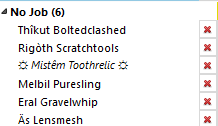
\includegraphics[width=0.32\textwidth]{Sec2Fig7}
  \end{center}
\vspace{-10pt}
\end{wrapfigure}
In a large enough fortress, trying to find out which dwarves are twiddling their thumbs is a
fantastically annoying chore. Luckily, we can simplify the task for ourselves by grouping our dwarves by
their current job. Going to the ``Group By`` drop-down menu and selecting ''Current Job'' will nicely clump
our dwarves by---what else---their current jobs. After a little bit of snooping, I'm able to figure out
what the problems are. We've got three jobless Miners with nothing to mine, a Woodcrafter (but really
Thresher) with nothing to process, a Metalcrafter with nothing to craft, and a Ranger with nothing to
haul. The Ranger will very soon find himself work, a spot of designation gets the Miners up and at it
again,\footnote{I cannot recommend the utility DFHack, and specifically its digv command, enough. It
makes digging designations \emph{so} much easier!} and I add some processing jobs to an idle Farmer's
Workshop. Bam; idle hands, managed! Ah, but what's this:

\fullfigure{Sec2Fig8}

Migrants! What are we going to do with them? After letting them get used to my fortress surroundings, I
open up the Dwarf Therapist, group by Migrant Wave, open up the new guys, and am now ready to do some
easy-to-make-out management; as an added bonus it'll tell you exactly how many dwarves you're getting
this season. Dwarves are loaded into the memory the instant the message appears, so they
don't actually have to be on your map yet for you to start working with their labor designations---a
neat feature.\footnote{Though it's generally reliable, when loading in dwarves from an auto-pause, the
program may occassionally miss a couple. If you want to ``play it safe'', wait until the first few
dwarves have made it onto your map.}

Now, whenever you group your dwarves the top row will consist of a collapsible group name and header, and
a series of labor boxes that, based on whether they'll filled out or not, tells you which labors have
been enabled within the group. Since these are new migrants and I haven't make adjustments yet, it
basically tells me what skills the random number god has gifted me with this migratory wave:

\fullfigure{Sec2Fig9}
\fullfigurecaption{Unfortunately Armok has not graced me with an armorer this season.}

By clicking on these headers you can enable or disable a labor for an entire grouping. Since we don't
want the new migrants idling, but haven't yet made facilities for most of them to use, let's do what we
always do when a new migrant wave arrives: mass designate stuff for them to do, in bulk. Well, it just so
happens that I've got a wall that I've been meaning to build, and there's quite a lot of fortress surface
that needs to be smoothed out (and don't even get me started on the many pictures of cheese that we need,
but lack!). So I click on the Masonry and Stone Detailing headers, toggle them on for the entire wave
(you can also right-click on the headers), commit, and voila---stuff for them to do!

Now, these are just two of the most immediately useful scenarios for which grouping comes in handy, and
there are quite a few more groupings that you can make and display. Additionally, if the correct option
is enabled, these groups carry across all of the views, not just the current one. To see a
demographic breakdown of your dwarves, group them by Age or Sex. To see which of your dwarves are
Legendary, group them by Legendary Status (or hit Highest Skill for a more inclusive view). To check up
on happiness, hit Happiness. To start working with Nicknames, hit Nicknames (this will prove useful in
\jump{Assigning Nicknames}, still ahead of us). To see what the chances of you
getting a Legendary Armorsmith are, hit Highest Moodable Skill. To sort them by Military Status, click
that, or Squad to check up on individual squads. To sort by Profession, hit profession.
% Avoid Total Assigned Labors and Total Skill Levels, however---these are bugged and the counts are
% clearly wrong.
Use Collapse All and Expand All to switch between detail levels without having to manually toggle groups;
for expedience you'll probably want to remember the associated \texttt{CTRL + <} and \texttt{CTRL + >}
shortcuts.

Groups are a great tool for discerning demographic information about your fortress, which is why they
work so well for spotting migrants---but as a sorting mechanism they're far from perfect. Dwarf
Therapist therefore supplements grouping with another organization scheme, sorting---the topic of the
very next section.

\newpage
\subsection{Using Sorts}
\label{sec:Using Sorts}
\begin{wrapfigure}{R}{0.35\textwidth}
\vspace{-20pt}
  \begin{center}
    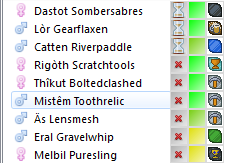
\includegraphics[width=0.35\textwidth]{Sec2Fig10}
  \end{center}
\vspace{-10pt}
\end{wrapfigure}
Let's now return to the problem of the six idling dwarves, and approach it with sorting in mind. When you
click on one of the column headers at the top of a view, it will sort the content in ascending order
against that column. The ``Current Job'' column is numerically sorted by the ``Job ID'', an internal list
number assigned to that job. There's no particular order to how Job IDs are assigned because there's not
truly superior logical way to organize them, but what's important to know is that idling is assigned a
value of ``-1''. Sorting the column once will put idlers at the bottom, then sorting again will flip it
around and bring them to the top---perfectly positioned for labor manipulation. Dwarves on break are
given a value -2 and, conveniently enough, are also displayed---on top of idle ones.

Sorting by happiness will list your dwarves by their numerical happiness level, grading your dwarves
down from ecstatic green to suicidal red---a far superior solution to the blunt and categorical Group
equivalent.

The fourth column in your view is the ``Profession'' column, which works in a similar manner to the
Current Job column, sorting by another arbitrary numerical system, the ``Profession ID'' list. The
arbitrary nature of the sort, and the large number of professional icons, makes it much harder to
recognize sorted professions from one another than grouped ones, so grouping is the clear winner when it
comes to this particular task. The professional listing does have one useful function, though, in that
it more immediately lists peasants at the top (or bottom) of the list.

Hovering over individual professions tells you how many dwarves have that labor enabled, and then
clicking on it will sort your dwarves by their experience and skill in that category. This is much
quicker and cleaner than performing the same operation with groups:

\fullfigure{Sec2Fig11}
\fullfigurecaption{Anyone can pick plants, but only true farmers can plant seeds.}

The ability to seamlessly list your dwarves by their competence at a task is one Dwarf Therapist's key
sources of utility, and has many obvious applications when you need to find dwarves for a task you have
in mind---like, say when building a marksdwarf squadron:

\begin{figure}[h!]
\centering

\includegraphics[scale=.9]{Sec2Fig12}
\end{figure}

You can go even further with \jump{Filter Scripts} and
\jump{Roles}, but those are advanced topics that we'll leave for later. If you right
click on a column you can change the sort method---this is a more advanced role-based capacity, and will
be discussed at length in the section \jump{Using Roles}.

\newpage

\subsection{Mass Designations}
\label{sec:Mass Designations}
In demonstrating the utility of grouping our use case was migrant wave designation, and in assigning our
new dwarves things to do we made use of Dwarf Therapist's groupwise designation tool. By clicking on a
group header you toggle a labor on for all legal dwarves in the contingent group; click on it again and
you will toggle it off. This is one of Dwarf Therapist's most apparent mass designation tools---we will
discuss these in detail in this section.

\begin{wrapfigure}{R}{0.4\linewidth}
\vspace{-20pt}
  \begin{center}
    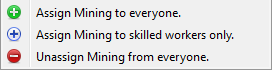
\includegraphics[width=0.4\textwidth]{Sec2Fig5-3}
  \end{center}
\vspace{-10pt}
\end{wrapfigure}
Groupwise designation is actually a subset of fortress-wide designation, which can be achieved with the
labor headers' right click menu, shown at right (the other options have to do with columnar sorting and
are covered in \jump{Using Roles}). Options one and three respectively toggle the
labor on or off for \emph{every} eligible dwarf in the fortress. The second option, meanwhile, is a smart
sort: it allows you to assign the labor only to those dwarves skilled in it (skill level Novice or
above), and it will disable it on dabblers.

The ability to designate bulk jobs thusly comes in handy in a number of different scenarios. In times of
war you can quickly toggle off dangerous jobs like Hunting and Plant Gathering, for instance, and when
you're finally getting around to dedicating a dwarf or a number of dwarves to a specific job you can
quickly eliminate that labor from all other stragglers. Assigning every instance of a labor is not so
immediately apparently useful but works well when combined with filter scripts, an advanced sort tool
described in detail in \jump{Filter Scripts}. Skilled labor assignment, meanwhile, can
be used to put those hunters and gatherers back to work after the danger has passed, or for reinstating
jobs accidentally deleted by careless labor editing.

\begin{wrapfigure}{R}{0.3\linewidth}
\vspace{-20pt}
  \begin{center}
    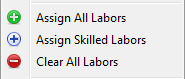
\includegraphics[width=0.3\textwidth]{Sec2Fig5-2}
  \end{center}
\vspace{-10pt}
\end{wrapfigure}
These three toggles comprise the laborwise mass designation tools and are complemented by similar
dwarfwise ones shown at right, also accessible with a right click (the other options on the menu are
covered at various other points in this guide). An option for assigning every labor is provided more for
the sake of parallelism than anything else---there are hardly any situations where you want a dwarf
working \emph{every} job, and in specialized labor subset views labor group designation is handled in a
more intuitive way by something else we're going to discuss shortly. Clearing all labors has the obvious
utility of allowing you to clean a dwarf's slate, saving you a number of clicks when you're dedicating
them to a labor. Finally, assigning all skilled labors does what it did in the laborwise menu but in
reverse, and can be used to ``de-dabble'' or otherwise ``reset'' a worker.

It should be noted that all of these designation tools respect the bounds of the view: that is to say,
they will not affect labors or workers that are not visible in the view. This behavior is useful if you
are filtering your dwarves, if you have removed certain benign labors (like Cleaning) from the view, or
if you are using a specialized custom labor subview. The triggers would better be named ``Assign All
Visible Labors'' and ``Assign Labor to all listed dwarves''.

\begin{wrapfigure}{R}{0.4\linewidth}
\vspace{-20pt}
  \begin{center}
    
\includegraphics[width=0.4\textwidth]{Sec2Fig5-4}
  \end{center}
\vspace{-10pt}
\end{wrapfigure}
By right-clicking on any labor box in the view you can toggle on or off that entire labor
tranche for the associated dwarf. This is an immense time-saver for those occasions when you have a
dwarf running a gamut of jobs---disabling or enabling the different hauling subtasks, for instance, or
enabling a gamut of tasks in a specialized labor subview (more intuitively suited for this tasks than
the full ``all labors'' trigger).

A similar labor-wise operation occurs when you select a group of dwarves and then attempt to toggle a labor on or off on any one them---this will toggle that labor on or off for all of the dwarves you have selected, which can be a useful operation when you're using role sorting as it allows you to more easily set mass labor behaviors for large, but unfiltered, groups of dwarves.

\newpage
\subsection{Assigning Nicknames}
\label{sec:Assigning Nicknames}

So you've spent a good ten minutes shifting around labors, building facilities, and generally getting
your latest migratory wave to work at the various things that need work in your fortress. You've
bootstrapped a metalworking industry, started making some potash, and are now weaving clothes. Feeling
content with yourself, and maybe just a little tired because it's somehow two in the morning and you've
been sitting here for five hours now, you save and log off so you can go get some sleep. In the morning
you wake up, pour yourself some cereal, check the time (still Sunday, thank god), stretch your arms, and
go right back to playing Dwarf Fortress. You open up Dwarf Fortress and...argh! What's this! Why are all
these silly peasants making crappy armor while your legendary armorsmith is idling! Who told that farmer
he could take over the cook's job! And most importantly, why is there still stone lying around
everywhere!!!

So perhaps playing Dwarf Fortress until two in the morning isn't good for your fortress (never mind your
sleep cycle). But there's another way to stay on top of the roles your dwarves are supposed to be
playing, one with which you can be relatively sure that, if you come back in a week's time instead of a
day's and have forgotten all of the various itty-bitty configuration details that the fortress survives
on, you'll be able to (more) easily pick them up again and keep right on playing. The solution is to 
name your dwarves.

Dwarven nicknames are often used rather jestingly by players, since you can name \emph{any} dwarf pretty
much \emph{anything}, even calling your King ``Giant Poo Poo Head" and your Great Potash Maker
``Unfortunate Accident". Dwarves don't know the difference and thus don't mind, but it's worth a cheap
laugh from the player if ``Giant Poo Poo Head" goes to clean up the blood stain left by the demise of
``Unfortunate Accident". However, they can actually be a pretty powerful tool if used right. By
nicknaming your dwarves by what their profession within your fortress is or will be, you'll be able to
more easily keep track of who they are when you bump into them in the labor manager or on-screen. Their
professional name might be ``Woodworker``, but to you they're ''Furnace Operator'', and using nicknames
allows you to keep track of that while their professional name catches up to their new role.

Let's look at one such fella for which a naming would be useful, a certain Medtob Swinwind.

\fullfigure{Sec2Fig13}

\begin{wrapfigure}{R}{0.35\textwidth}
  \begin{center}
    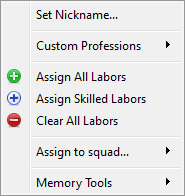
\includegraphics{Sec2Fig14}
  \end{center}
\end{wrapfigure}
Mebtob has a few assorted skills---he's an adequate Tanner and Fish Cleaner, and a Novice Fisherdwarf and
Fish Dissector. However, none of these skills are really useful to me: I've got enough fisherdwarves and
fish cleaners already,\footnote{Because of a bug, fish stocks do not replenish, which means that they
will inevitably go bust, leaving your fishery workers with nothing to do.} tanning is only useful every
once in a while, and fish dissection is a near completely worthless skill. What I \emph{do} need,
however, are some leatherworkers---I just bought a shipment from a caravan, and want to turn it into a
complete set of backpacks, waterskins, and quivers for my military to peruse. Unfortunately the random
number god has not blessed me with any professional leatherworks---which is fortunate for Mebtob, since
he's now going to move past peasanthood to become the fortress leatherworker.

For now, though, he's still a regular old fish cleaner, and if you bump into him in the hallway or look
at him in Dwarf Therapist after a week away or a really long night, you won't have a clue what he's there
for. So to make that job easier, let's give him a nickname. Right click on Mebtob to bring up the same
personalization menu we discussed a section earlier. For now we want ``Set Nickname'':
\newpage

\begin{figure}[h!] \centering
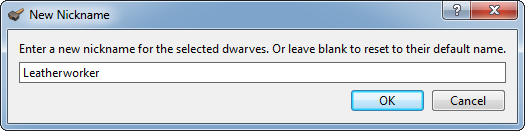
\includegraphics{Sec2Fig15}
\end{figure}

New nicks are actually treated the same way as labor changes: once you've chosen a new nametag for your
dwarf to go by and clicked on ``OK'', the name change will be added to the Pending Labor Changes dock,
awaiting committal:
\begin{figure}[h!] \centering
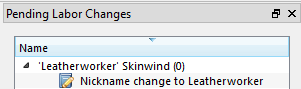
\includegraphics[scale=1]{Sec2Fig16}
\caption{Ah yes, compatriot ``Leatherworker Skinwind''.}
\end{figure}

Commit the change, and you shall confuse the role this dwarf plays no longer.

That concludes our discussion of Dwarf Therapist's basic labor management tools. We will cover many more
advanced features in the \jump{Advanced Features} section of this guide, but for now
let's examine another aspect of the program: the options menu.

\addendum{
\subsection{Addendum: Managing your Animals}
While most of the views in Dwarf Therapist besides
the labors view are non-interactive, two are. One is the Animals view, worth mentioning
here; the second, the ``Roles'' view, is discussed in \jump{Using Roles---The View Method}. The Animals
view provides information on the name (duh) and owner of the creature, their ``profession'' (really whether
they are children or adults), their training level (nothing is displayed if they are tame), whether or
not they are designated for or can be butchered, whether or not they are in a cage, and their physical
attributes. I say that this menu is interactive, and it is: non-wild, non-pet creatures can be
designated for butchering here. This allows it to replace the in-game Animal Status screen, provided
that you don't try to tame any wildlife, as this cannot be done through Dwarf Therapist.
}

\newpage
\section{Options}
\label{sec:Options}

The Options menu is available from a few different places: either a button on the main taskbar, through
the ``File'' menu in the main menu, or with the \texttt{Ctrl + P} hotkey. This brings up a menu:
\fullfigure{Sec2Fig17}

The options menu is extremely well-documented: if you're ever at a loss for what a particular checkbox
or radio button does, hover over it and look for its description in the text box at the bottom of the
dialogue. It's all quite intuitive and well-explained, so instead of wasting a ton of time and space
describing it, I invite you to explore the menu, and then come back to here.

Good? If you're still interested in fiddling with the options, see the upcoming section. If not, skip
ahead to the next part of this guide, \jump{Advanced Features}.

\newpage
\subsection{Formatting Your Display}
\label{sec:Formatting Your Display}

\legacy{
A big problem I had with the default configuration of past versions of Dwarf Therapist is its affinity
for gloss over informational density---non-functional fade-out boxes and headers and dividers that eat
up tons of screen space were present, while several options that enhanced information display were not.
More recent version of Dwarf Therapist have implemented some of the suggestions in this section by
default, making some of these changes redundant, but this section is still provided to the reader as a
reference. }

% This section is left to the reader as a demonstration of the program's robust options menu.
% Since most of these changes no longer need to be made the illustrations for this section are from legacy
% versions of the program.}

\fullfigure{Sec2Fig18}
\fullfigurecaption{My horizontal scroll bar at the beginning of this exercise.}

\noindent \textbf{Remove Spacers}

To remove the spacers from the long-form Labor view, peruse the \textbf{\nameref{sec:Screens Tab}}. Drop
in the ``Labor NO SPACERS`` view from the menu and then delete the old one. Of course having ''NO SPACERS''
stare at us is quite annoying; we'll look at ways to fix this later in this guide.\footnote{Note that as
of version 20.6 Dwarf Therapist now ships with the very view solution first presented in this guide as
an alternative option to the default: check the ``Labors Alt'' option.}

\fullfigure{Sec2Fig19}

\noindent \textbf{Turn off Gradient Shading on Headers}

To remove the gradient shading in the column headers and return them to plain coloration, uncheck
``Gradient Shade Column Headers'' in \texttt{Options > Grid Options}.

\fullfigure{Sec2Fig20}

\noindent \textbf{Turn off Gradient Shading on Cells}

To remove the gradient shading present on table cells that are toggled on, uncheck ``Gradient Shade Cells''
in \texttt{Options > Grid Options}.

\fullfigure{Sec2Fig21}

\noindent \textbf{Synchronize Scrolling between Views}

To enable this feature, check ``Synchronize View Scroll Positions'' in \texttt{Options > Grid Options}.
This adds some functionality to your views, preserving the current scroll position between them and
letting you examine a single dwarf (or if they're sorted the same way, a group of dwarves) through the
lens of multiple different views. They don't have to be sorted the same way for this to work, though
occasionally it near-misses (bringing you to the dwarf just above the one you care about in the view).
\vspace{12pt}

\noindent \textbf{Highlight Highest Moodable Skill}

To enable this feature, check ``Highlight moodable cells in labor/skill columns.'' in \texttt{Options >
Grid Options}. This one's optional: it gives you extra information, but knowing what moods your dwarves
are likely to have isn't terribly useful since the selection is random, and you can get the information
at a glance through a Group. Though it doesn't say it, this option also highlights dwarves that are
legendary because of a mood with a different colored box. You can change the colors in \texttt{Options >
Grid Colors}.

\fullfigure{Sec2Fig22}
\fullfigurecaption{Moodable in green, already mooded in brown.}

\noindent \textbf{Show Highest Moodable Skill in Tooltip}

To enable this feature, check ``Show Highest Moodable Skill in Tooltip'' in \texttt{Options > Tooltip}.
This will add a ``Highest Moodable Skill'' entry to the dwarf tooltip---no real reason not to have it.
\vspace{12pt}

\begin{wrapfigure}{R}{0.3\textwidth}
\vspace{-5pt}
  \begin{center}
    
\includegraphics[width=0.3\textwidth]{Sec2Fig23}
  \end{center}
\vspace{-10pt}
\end{wrapfigure}
\noindent \textbf{Make the Main Toolbar More Compact}

To shrink the main toolbar a bit so that it doesn't take up so much vertical room (and thus give your
view and your docks more of it), uncheck the ``Show Toolbar Text'' option in \texttt{Options > General}.
\vspace{12pt}

\begin{wrapfigure}{L}{0.25\textwidth}\vspace{-20pt}
  \begin{center}
    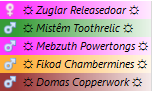
\includegraphics[width=0.25\textwidth]{Sec2Fig25}
  \end{center}
\vspace{-15pt}
\end{wrapfigure}
\noindent \textbf{Highlight Nobles}

To turn this feature on, hit ``Highlight Nobles'' in \texttt{Options > Nobles}. The default color is
orange, and you can further pick specific colors for specific roles. Personally I set chief medical
dwarves to dark red, bookkeepers, managers, mayors, and brokers to default, royals to magenta, and
military types (militia leaders, champions) to dark green.
\vspace{12pt}

\noindent \textbf{Role Information in Labor Columns}

To turn this feature on, hit ``Role Information in Labor Columns'' in \texttt{Options >Roles}. We've barely
talked about roles so far, and they're covered in-depth in the section on them, thoughtfully titled
\jump{Roles}. For now it's just more information for you to peruse.\
\vspace{12pt}

\noindent \textbf{Move, or Remove, your Docks}

Docks are a very useful thing, displaying useful information in a compact form. However, if you want to
make the most use of your space: go without. Removing all docks from the right side of the screen so that
the edge of the view window is now plum against the right edge should be enough to let you see the
entirety of the grid on a moderately large screen.

\fullfigure{Sec2Fig26}
\fullfigurecaption{On my (21-inch) monitor, it was enough to get rid of the scroll bar completely.}

If you want to get rid of the scroll bar but want to keep your docks, too, another option is to place
them at the bottom. This is a dock-heavy option, however, because the docks are not optimized to use
horizontal space well---so giving the Pending Labor Changes the entire lower fourth of the screen is no
better than giving it the same amount of space, vertically, on the sidebar.
\vspace{12pt}

\noindent \textbf{Remove the Main Toolbar}

The main toolbar is very skinny: if, like me, you have space on the right edge (or can spare a sliver
off the top), you can simply and safely stick it there. But if you want to reclaim that last ounce of
screen space, by all means, remove it: all of its commands are hotkeyed anyway.
\vspace{12pt}

\noindent \textbf{Play with Fonts, Spaces, and Font Sizes}

If this still isn't enough to get rid of the horizontal scroll bar, and you really, really want to get
rid of it, you can play around with the fonts, font sizes, spacer options, and grid sizes in
\texttt{Options > Grid Options}, and lower the sizes of things until the bar is no more. Obviously, the
smaller the font and grid size, the harder it is to read information of the utility---even reducing it
from 16px to 15px has a noticeable effect.
\vspace{12pt}

Here is what my display looked like at the end of this exercise:
\fullfigure{Sec2Fig28}

Cleaner, more informative, and most importantly: no horizontal scroll bar!

\newpage
\part{Advanced Features}
\label{sec:Advanced Features}

In this section of the guide we're going to really dig into Dwarf Therapist, working with powerful
elements of the program that aren't as immediately apparent as toggling labors on and off, giving stuff
nicknames, and other such simple and obvious applications.

\section{Roles}
\label{sec:Roles}
\subsection{What's in a Role?}
\label{What's in a Role?}
So far we've mentioned ``roles`` and the ''role'' they play in  Dwarf Therapist only in passing. Since we're
now going to discuss them in more detail, the first question we have to ask is, what's in a role?
Have you ever had two miners work side-by-side from the very beginning of the game, but
discovered that one reaches legendary status before the other? This happens when one dwarf is
better adapted to that role than his fellow, and the differences between them become increasingly
obvious over time. ``Roles'' is Dwarf Therapist-speak for the holistic weighing of the various
elements of job performance, of which skill is only the most immediately visible and obvious element.
Thus in order to understand what roles are, we must first get comfortable with what these elements are,
and where they come from.

\textbf{Attributes} are, subjectively speaking, the most important hidden role modifier. No two
dwarves are alike, and all dwarves have certain attributes that are attached to them from
birth.\footnote{Attributes, alongside appearance modifiers, are inherited through dwarven genetics.}
Where one dwarf might be naturally weak have superb spatial sense, another might lack analytical
ability and be susceptible to disease, but be unnaturally strong. These attributes themselves fall into
two categories, physical and mental; they can be assessed under the ``Attributes'' view, and they're
described in detail on the DFWiki: \url{http://dwarffortresswiki.org/index.php/DF2014:Attributes}. Since
they're pretty important for understanding roles, here's a quick list of the ones that affect job
performance:\footnote{It should be noted that all creatures, not just dwarves, have attributes (for
instance, the attributes of animals attached to your fortress are visible on the ``Animals'' view). The
attributes of creatures that are not tied to your fortress---wildlife, unwelcome visitors, hostile
sapient creatures, caravan traders and guards---will be hidden from you.}

\boldlist{\indent Physical Attributes}

\boldlist{Strength} Alters the damage done in melee (increases velocity
of weapon swings), increases muscle mass (thicker muscle layer also resists damage more), and increases
how much a creature can carry. Higher strength also increases the speed with which a creature, even a
naked creature, may move. Movement speed is important for pretty much every task, but to a varying
degree.

\boldlist{Agility} This attribute increases the speed at which a creature works in the same way as
strength -- a creature with maximum agility and strength can move around three times faster than a
creature with minimum agility and strength.

\boldlist{Endurance} Reduces the rate at which dwarves become exhausted, important for physically
demanding tasks.

\boldlist{Toughness} Reduces physical damage. Used by physically demanding tasks.

\boldlist{\indent Mental Attributes}

\boldlist{Analytical Ability}

\boldlist{Focus}

\boldlist{Willpower} Willpower directly reduces exertion and pain effects, useful for physically
demanding tasks.

\boldlist{Creativity}

\boldlist{Intuition}

\boldlist{Patience}

\boldlist{Memory}

\boldlist{Linguistic Ability}

\boldlist{Spatial Sense}

\boldlist{Kinesthetic Sense} Most skills involving any movement at all (lots of them), and many
non-skilled tasks as well are affected by Kinesthetic Sense.

\boldlist{Social Awareness}

\vspace{12pt}

Physical attributes will increase or decrease over time, depending on whether a dwarf uses
or doesn't use them in their day to day tasks. Thus your Miner will become very tough and very strong
while working on the job, and would make a good recruit for your military in their
next, ahem, role.

Another modifier is a dwarf's \textbf{personality traits}. For the most part
personality traits only affect social skills and appointed jobs that involve working with others -
expeditions leaders, managers, brokers, and mayors use them, as do high nobles. There is one,
perseverance, that is thought to affect the length of breaks that your dwarves will take, and might thus
be important for all skills---your dwarves will obviously do less work overall if they're
always on break. However, Toady has never confirmed this.

The final hidden element of a dwarf's role is his or her \textbf{preferences}. Dwarves
have innate preferences for certain items, materials, organisms, and even colors and shapes (I want my
coffin to be a \emph{yellow square}, you hear me!). Dwarves like seeing things they like---they'll get a
happy thought from it---and they like working with them even more, producing above-average quality goods
when working on items or with materials that they like. For this reason a dwarf that likes beds will
make a better carpenter than a dwarf that like breastplates and vice versa. Having the right sort of
preferences can be an important bonus in a dwarf's work, meriting weight in the role calculations.

Now that we've examined all of the elements besides skill that are weighed into roles, the next logical
question is: how are role numbers calculated? As it turns out, this is not a trivial question.
There are, essentially, three ways of ``thinking about''---and hence using---roles. Let's first examine
th default behavior, which can be seen and modified in the ``Roles'' Options menu (\texttt{Options >
Roles}):
\fullfigure{Sec3Fig1}

\newpage
Dwarf Therapist takes a dwarf's attributes, skills, traits, and preferences and weighs the ones that
matter for a certain labor by the amounts inputted here. It then performs a \textbf{cumulative
distribution function} on the results, giving you how fit that dwarf is for that role as a percentage
calculated against the \emph{current dwarves in your fortress}. The result of this statistical trickery
is that while the result is a \emph{current} rating, it's \emph{non-transferable} (a 75\% rating in one
skill is not directly comparable to a 75\% rating in another) and \emph{non-preservable} (role ratings
will resettle every migrant wave, or every time a child grows up). For the purposes of this guide, I call
this rating \textbf{skill rank}.

Changing the second option in \texttt{Options > Roles}, ``Default Skill Weight'', to 0 removes it from the
equation. With skills no longer counting for anything, the role rating now shows what I refer to as
\textbf{basal compatibility}---the results of a CDF crunch of your dwarves' attributes, traits, and
preferences alone. This is a useful view of your fortress ``in retrospect'', as you might discover that the
weaponsmith you appointed from scratch in wave one is completely outclassed by several dwarves in waves
two, three, and four. Of course by that point that dwarf would have put on so much distance in terms of
skill that it doesn't matter anymore---but it's still an interesting statistic to know. It's also much
less statistically sharp than skill rank is, because base stats don't vary nearly as much as skill does.

The last and most useful function that roles serve is one that answers the question "Which of these
dwarves will reach legendary status the quickest?" In such a distribution an unskilled dwarf with minimum
stats will be rated at zero percent, an accomplished one with middling stats would be a fifty, and that
legendary +5 dwarf with maximum stats and perfect preferences and whatnot would be a one hundred: a
\textbf{true role rating}. So, how do you turn this wonderful ranking on?

Well\ldots you can't. It's a pipe dream. There are simply too many variables involved in job completion
length and skills gain and no one's ever fully done anything beyond rudimentary research on the topic -
it's very complicated and not nearly as glamorous as combat weapon penetration rates. Even the weights
that the program uses are the result of conjecture---there's just not enough !!SCIENCE!! to base the
whole thing on as of now, and that's the reason that we have to use skill rank, drawbacks that it has,
as a substitute.

\subsection{Using Roles---The Sort Method}
\label{sec:Using Roles}

\begin{wrapfigure}{R}{0.3\textwidth}\vspace{-22pt}
  \begin{center}
    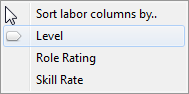
\includegraphics[width=0.3\textwidth]{Sec3Fig2}
  \end{center}
\vspace{-15pt}
\end{wrapfigure}
There are two distinct ways to go about applying role ratings, one involving sorting, one involving a
different view. I will describe them in order of preference---sorting settings first, the ``Roles'' view
second.

We've talked before about the utility of clicking on the labor headers and having your dwarves sorted in
ascending order of experience. But did you know you can actually change this behavior? Indeed,
right-clicking on anywhere on the labor headers will bring up a menu that allows you to change the
current labor sorting behavior, as seen on the right.\footnote{You can also change the sorting behavior
of the dwarf column, to sort by ID (a somewhat useful alternative to grouping by migrant wave) and age
(useless). Unfortunately, it will not save this behavior, and attempting to reverse the sort will send it
right back into alphabetical order.}

The first option, Level, is the default option, and that makes sense. The third option is pretty much the
same as the first, except that skill rate (which the amount of skill gained every time a labor in that
category is completed) is modified by, you guessed it, the dwarf's role, and so will vary a little from
straight up experience level---but experience is still the most important indicator of relative skill
gain, so it won't change too much. However, the one we want right now is Role Rating. Click on it. Now,
whenever you sort a column, the dwarves will be listed by their adeptness for that labor. Assuming you
turned the role tooltip display on, as we did in \jump{Formatting Your Display}, then
you can hover over a labor box to see the exactness of the match---if you skipped that section, you can
toggle the behavior on now by going to \texttt{Options > Roles > Show role information in labor columns}.

If you play around with sorting the columns now, you will notice two things. The first is that dwarves
with the labor enabled and those with it disabled are considered, and listed, separately from one
another: under the ascending sort, dwarves active with that job come first, followed by those that are
not. The second is that in terms of basal compatibility skill is (mostly) irrelevant; beyond the fact
that we took it out of the calculations in the previous section, this indicates that physical attribute
gain from performing labors that use that attribute is simply not that high. And so it may be that your
primary mason is buried nearer to the bottom of the list, with a compatibility of 14\%, with a long list
of mostly dabbling dwarves that outrank him:

\fullfigure{Sec3Fig4}

In this case the reason that the dwarf that became my chief mason was so incompatible with his job is
that he was part of my starting seven, and so his attributes were random---and the random number god did
not favor me in this case. It's important, however, to realize when basal compatibility is important and
when they are not. While basal compatibility will tell you which of two comparable dwarves would be
better at a certain job, they are no replacement for hard-won experience, and so that dwarf, incompatible
though he may be, is many times better than any of the laymen that pretend to also do his job. Once you
put three or four levels of experience points between two dwarves, their roles lose all relevance.

So then, when are roles important? As it so happens, my fortress just experienced a migratory wave, and
something that my fortress critically lacks right now is metalworkers. I'm a big believer in expensive,
well-decorated furniture for my dwarves, and I've got a skilled gem setter running around encrusting beds
in locally-mined sapphire, but he's not keeping up with the demand. I have a lot of extra fuel, some gold
bars, and a couple of metalsmith's forges idling around, so I decide that the solution to my problem is
to put two of these new migrants to work as dedicated metalcrafters, studding every piece of jewelry they
can get their hands on in gold. Since no one has a skill advantage in this arena (my fortress has zero
metalcrafters), and all but two of my dwarves are pretty much useless anyway, I want to pick out the best
two dwarves available from this wave. How do I go about doing it? By combining two things we've learned
so far, grouping and sorting, with a third---roles.

Try doing this exercise yourself---you need not even have a fresh migrant wave. First, group your dwarves
by migration wave, collapse them, and open the latest wave. Now, with the sorting method set
appropriately, hit ``Metalcrafting'' to sort these dwarves by role score. Now look down your list.

\fullfigure{Sec3Fig5}

In my case, the first dwarf on the list was an Adept miner with a score of 98.1 percent; but mining is a
useful skill and I'd rather he cut rock for the fortress, so I keep going down. The next option is
better: a ranger whose only real usable skill is hunting, and a farmer with some assorted non-essential
skills, both of whom are easily replaceable. I right click on their names and hit ``Clear all Labors'' to
quickly wipe their workloads, designate metalcrafting for the pair, and then hit ``Commit'' to send the
changes to the game. I even give them nicknames, to be extra sure I won't forget about them:

\fullfigure{Sec3Fig6}
\fullfigurecaption{Notice the change is sorting behavior to reflect changes in labor designation.}

And voila---we are done. Now we take a quick look at how this problem can be approached using the
``Roles'' view.

\newpage
\subsection{Using Roles---The View Method}
\label{sec:Using Roles---The View Method}

Another way to tweak your dwarves using roles is to use the ``Roles'' view.

\fullfigure{Sec3Fig10+}

This is one of the secondary views that is open by default when you first install the program. The
difference here (besides the fact that this view uses the old labor organization system) is that instead
of displaying dwarves' labor preferences, this view displays their role ratings, allowing you to
manipulate their labor preferences based on role without having to change your sorting settings. This has
the advantage of not having you to mess with your sorting settings, but the disadvantage of having to
switch to another view.

Other than the difference in the up-frontness of the information, using the view method to make
role-informed labor changes isn't all too different from using the sort method---group up your
migrants, click on the column to sort the role, then pick an acceptable candidate from the bunch.
Overall, I prefer dealing with sort settings to dealing with another view, so in my games I use the sort
method---but you are free to chose whichever appeals to you more.

In either case, our end result is that we have now committed two well-suited dwarves to their new
tasks \emph{almost} flawlessly. But there are other, similarly replaceable dwarves also in the fortress
that would make better candidates for this job but aren't in this particular migratory wave, but hunting
them down is a pain. I could find the best-suited dwarves in the \emph{fortress} by turning off grouping
and then sorting the column, but then I'd bump into another problem: which dwarves are replaceable, and
which ones am I training up or holding onto with certain roles in mind? In this respect, your tools are
crude---\emph{maybe} you remember exactly or can deduce from the labor settings what role each dwarf is
set for, but in a fortress of 200, you probably don't. In large fortresses with many industries, it's
simply not possible to easily keep track of so many variables at once.

We can solve this problem by using nicknames aggressively, designating all dwarves committed to a task
with a nick, and then using the ``Has Nickname'' grouping in the view. Setting so many nicknames is
tedious, however, and if you don't like using them then you're out of luck. Or are you? There is another,
more powerful solution that will come later in this guide: filter scripts. For more details on this, see
\jump{Filter Scripts} for the scoop.

Assigning jobs based on role ratings is fine and all, but what if there was something you could do that
would allow you to do this automatically? \jump{Optimization Plans}, which we'll discuss much later in
this guide, do just that.

\addendum{

As mentioned in this section, any role which has skilled labors associated with it will automatically
allow you to toggle those labors through the role's role rating column, and you can toggle multiple
labors this way. This capacity often comes in handy when doing what we will be doing in the next section
of this guide, defining our own grid views. See \jump{Custom Grid Views} for more.

}

\newpage
\subsection{Creating Custom Roles}
\label{sec:Creating Custom Roles}

%\begin{wrapfigure}{R}{0.3\textwidth}\vspace{-22pt}
%  \begin{center}
%    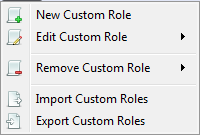
\includegraphics[width=0.3\textwidth]{Sec3Fig7}
%  \end{center}
%\end{wrapfigure}

If you right click on ``Roles'' on the menu bar it will bring up a menu with several role-modification
related entries on it. Dwarf Therapist allows the creation of custom roles through
this dialogue, and you can also export and import other player's custom roles definitions. If you don't
like a default role, you can overwrite it by building and saving a custom role with the same
name.\footnote{You can also do this by exiting Dwarf Therapist and browsing to and modifying the
\texttt{game\_data.ini} in the program's install directory: see \jump{Game Data} for
more information. A word of warning: your changes will not be preserved should you update Dwarf
Therapist.} Click on ``New Custom Role'' and it should bring up this dialogue:

\fullfigure{Sec3Fig8}

\newpage
This is the editing interface for creating a custom role, and clearly demarcates the four components of a
role. There is a scripting option available---this is a plug-in for \jump{Filter
Scripts} that we'll talk about later. And finally, the italic text at the bottom of the window tells us
that roles changes will not be read in until you reread your dwarves, so we will have to do so after
we're done here.

% \legacy{
% Dwarf Therapist ships with a pretty comprehensive role library---it even has lawdwarf (weak) and liar
% options, and provides role information for jobs that are not implemented into the game, such as alchemy.
% However, there is one feature that it lacked at the time of this guide's writing, and that was a role
% setting for haulers. Such a role definition, based on the work done in this section, is now provided by
% the program as an example of a custom role---we will proceed to build it here. }
Dwarf Therapist ships with a pretty comprehensive role library---it even has lawdwarf (weak) and liar
options, and provides role information for jobs that are not implemented into the game, such as alchemy.
However, there is one role definition that it lacks, and that is a role setting for haulers. Ye peasants
do their job best when they're quick and strong, but there's no role for such a thing available! The
solution, of course, is to write our own.

Start by copying role settings from a similarly physically demanding job---say, mining. Scroll down to
mining in the ``Copy From'' menu (or hit M while the menu is active to get there more quickly) and click
``Copy''. This will copy all of the role settings for minters into the dialogue. Our haulers need not be
lovers of picks, so let's remove it from the Preferences screen---right click on it and hit "Remove
Selected". Skills are irrelevant, too (especially for an unskilled hauler), so remove that as well.
Actually, for a hauler that's going to be carrying pretty much everything in the fortress back and forth,
preferences are unimportant---they'll bump into pretty much everything---so let's drop stone, too.

Hauling is an unskilled job, so the only things that matter for it is the speed and endurance of the
dwarf. That means that the Strength, Endurance, Willpower, Agility, and Toughness attributes are at a
premium, and the rest can be gotten rid of. The only Trait that matters to use is self-discipline---don't
want them taking two-season breaks, after all---so let's add that into the mix, too. And, of course,
let's give your new role a name: ``Hauler'' seems appropriate.

This is what the important settings in the interface should look like at the end of our little exercise:

\fullfigure{Sec3Fig9}

Hit ``Save'' to save your new custom role. Now, whenever you go to the Custom Roles dialogue box, hovering
over ``Edit Custom Role`` or ''Delete Custom Role'' will give you the option to perform that action on your
new role. Custom roles can be used in custom views and in labor optimization---we'll see an application
for them later---but cannot yet be bound to custom professions or to labors.

\subsection{Exporting and Importing Custom Roles}
It's also possible to export custom roles, which creates a Dwarf Therapist export file (\texttt{.dtp})
that can saved and then passed along to another installation of the utility by importing it. You can
export your custom roles and then upload them on the web (preferably the Dwarf Fortress File Depot:
\url{http://www.dffd.wimbli.com/}) to share them with other players, or you can download one from the web
and then import them into Dwarf Therapist so that you can use them too.

\section{Custom Professions}
Dwarf Fortress has a \emph{lot} of professions, and even more skills, available to your dwarves. In fact,
learning what each profession and skill corresponds to is one of the hardest part of learning to play
the game, because there's just so many of them. You can add to this sprawl by creating your own
professions, assigning multiple labors to one unified profession. This ability has its uses, and in this
section we're going to use it to unify hauling labors.

Whether your dwarf is hauling around sacks or focused on their primary task is usually an all-or-nothing
thing: either they're committed to their job, or they're not. It's not very useful to have dwarves only
perform \emph{certain} hauling tasks, unless you're getting into the extreme end of fortress management
and optimization, so most players of the game have them either all on or all off on a dwarf-by-dwarf
basis. We're also going to assign the ``Hauler'' role that we built in the previous section,
\jump{Creating Custom Roles}, to this new, unified profession.

\subsection{Creating Custom Professions}
\label{sec:Creating Custom Professions}
\begin{wrapfigure}{L}{0.36\textwidth}
\vspace{-20pt}
  \begin{center}
    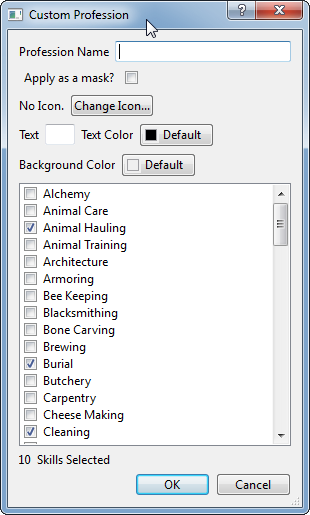
\includegraphics[width=0.36\textwidth]{Sec3Fig10}
  \end{center}
\vspace{-15pt}
\end{wrapfigure}
The dialogue for creating custom professions is located in one of two places, and you can get there
either by hitting ``Create Custom Profession'' at the bottom of the Custom Professions dock, or by right
clicking on a dwarf, going to ``Custom Professions``, and hitting ''New custom profession from this dwarf''.
This second method starts you off with the labors that that dwarf had enabled checked, and so is faster
if you have a dwarf already set to the labors you want---and after a quick profession sort I discover
that I do, in fact, have a peasant hanging around my fortress, so I open it up off of him. Lo and behold,
the ten hauling ``subskills`` are already selected. I name the profession ''Hauler'' and give it a red circle
icon, one of the spare ones in the utility's default set that's not already used by a professions. To
make it clearer that this icon is for haulers, I'm going to use the text and text coloration option
provided in the window to draw a white H over my icon. You can also add a background color, but the
regular icon set keeps a transparent white background, so I will too. I hit ok and the profession is now
listed under ``Custom Professions'' in the Custom Professions and Icons dock. To make it appear in the
display, you have to commit your changes and reload your dwarves.

To work the way we intended, make sure you don't check the Mask option in the window---this will change
the behavior so that the custom profession only masks the dwarf's ordinary profession, and it will not
allow you to make designation changes. You can remove a dwarf's custom profession designation with "Reset
to default profession" and then a commit to the game.

\begin{wrapfigure}{R}{0.40\textwidth}
\vspace{-10pt}
  \begin{center}
    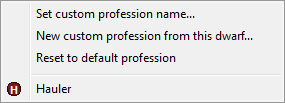
\includegraphics[width=\linewidth]{Sec3Fig11}
  \end{center}
\vspace{-10pt}
\end{wrapfigure}
You can create a mask more directly by right clicking on the dwarf and then going to "Set custom
profession name" under the custom professions menu, and then inputting a name: once committed this will
change the dwarf's profession to a custom one. This is a by-dwarf operation that basically mirrors how
custom professions work within the game, replacing the dwarf's professional name with the new string but
not changing anything else, without labor assignments or a custom icon, and with no facilities for
transferring the profession to other dwarves. Thus it's like a nickname applied to the dwarf's
profession, and in fact provides the same ``who's this dwarf?'' functionality that we previously used to
make nicknames useful. However, since nicknames can be more easily seen at a glance within the Dwarf
Therapist utility (and don't get in the way of this feature's more advanced version), I recommend
sticking with them for this function. For more on custom professions, in particular a part of
their utility that we're not yet ready to cover here, see \jump{Super Labors}.

\subsection{Exporting and Importing Professions}
\label{sec:Exporting and Importing Professions}
\begin{wrapfigure}{R}{0.425\textwidth}
\vspace{-20pt}
  \begin{center}
    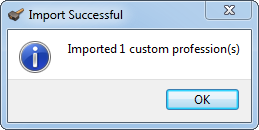
\includegraphics{Sec3Fig12}
  \end{center}
\vspace{-15pt}
\caption{Binmaker extrordinare.}
\end{wrapfigure}
Custom professions is actually one of the two Dwarf Therapist features we discuss (alongside
nicknames) that are present within the base game, although custom professions have less utility within
the game---they simply replace the dwarf's professional name. If you want to assign the same profession
to multiple dwarves you have to do so manually, retyping it in each time. If you assign a custom
profession to a dwarf within the game, but don't import it, his professional name will change in Dwarf
Therapist but nothing else will (essentially the same as setting a mask). To make the profession more
available to Dwarf Therapist, allowing you to more easily assign it to multiple dwarves, give it an icon,
and use it as a labor designation shortcut, you have to import it. To do so, hit \texttt{File > Import
Professions from DF}---it'll give you a quick confirmation window telling you how many professions you've
imported.

Much as with roles, custom professions can be made within the utility and exported, or taken from someone
else and imported---this is actually going to be a common theme between the various customizable
functions we're discussing in this section of the guide. There are even dialogues that let you pick and
choose which professions you want to export or import. Both options are available from the \texttt{File}
menu.

\addendum{

\section{Addendum: Custom Icons}
\label{sec:Custom Icons}

If for some reason you do not like the default professional icon associated with any particular
profession, you can change it to whatever icon you like by right clicking on the it and hitting
``Customize''. You will be brought to a ``Custom Icon'' window very similar to the ``Custom Profession''
window, but with the profession name grayed out and the labor toggles not present (since you're only
dealing in iconographry). Any edited professional icons you use will be recognized by the program as
custom icons, and presented as such in the ``Customizations'' dock, where you can edit or delete them.
Note that custom professions are treated by the program as something rather more comprehensive than just
a custom icon, and will show up in this dock as ``Custom Professions''---the icons you create for them
will not be listed separately.

}

\newpage
\section{Custom Grid Views}
\label{sec:Custom Grid Views}

\legacy{
Probably the most important immediate consequence of the writing of this guide was the introduction of
the improved ``Labors'' view as the default view in Dwarf Therapist. This view was built over the
course of this section, using Dwarf Therapist's custom grid view capacity. The way it was built, and the
thought process behind the changes, is presented here.
}

\begin{wrapfigure}{R}{0.35\textwidth}
\vspace{-20pt}
  \begin{center}
    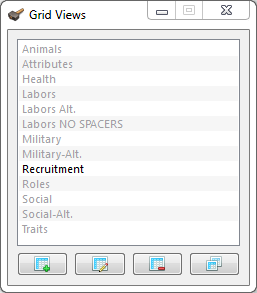
\includegraphics[width=\linewidth]{Sec3Fig13}
  \end{center}
\vspace{-50pt}
\end{wrapfigure}
Unlike the rest of the advanced utilities we're discussing in this section of the guide, custom grid
views can only be created and edited through the associated dock, so if you don't have it open already do
so at least for the duration of your editing.

Inside the dock you will find the grid views that the utility comes pre-loaded with, but they will be
grayed out. You can create a new, editable grid view in one of two ways: either by hitting "Add New Grid
View", which gives you a blank, or by right clicking on and copying one of the views that is already
hardcoded in, which will generate you an editable copy of the view.\footnote{Note that the grid views
that come hard-coded with the utility cannot be deleted.} At right you can see what the grid views dock
looks like with one custom view, ``Recruitment'', already defined.

Try hitting the ``Add a new grid view'' button and you will be brought to an empty grid view creation
dialogue:
\vspace{24pt}

\fullfigure{Sec3Fig13+}

The grid view creation dialogue organizes its columns into ``sets'', which are organizatory\ldots
sets\ldots of columns of one color. If you try to create grid view columns without sets to place them in,
Dwarf Therapist will complain to you. You can set the name and background color of a set, the latter of
which is made the default background color for all columns in the set. Also note that you can make
animal-specific views, like the ``Animals'' view packaged with the program by default. The main feature,
however, is the individual columns themselves.

\begin{wrapfigure}{R}{0.35\textwidth}
\vspace{-20pt}
  \begin{center}
    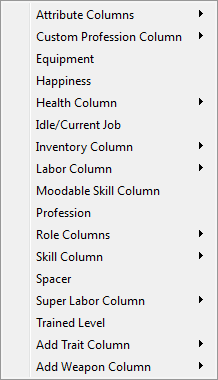
\includegraphics[width=\linewidth]{Sec3Fig13+1}
  \end{center}
\vspace{-100pt}
\end{wrapfigure}

\boldlist{Attributes} This is where you will find the attribute columns used in the default
``Attribute'' view.

\boldlist{Custom Professions} This option allows you to display labor toggles for the super-labors
associated with these professions (see the next section, \jump{Super Labors}).

\boldlist{Custom Roles} This option allows you to display role ratings for custom roles you've defined,
exactly like you can with regular, pre-defined roles.

\boldlist{Equipment} A special ``Equipment'' column present by default in labor views.

\boldlist{Happiness} A special ``Happiness'' column present by default in the labor views.

\boldlist{Health} This is where you will find the health information columns used in the
default ``Health'' view.

\boldlist{Idle/Current Job} A special ``Current Job'' column present by default in the labor
views.

\boldlist{Inventory} This is where you will find the military inventory information columns used
in the default ``Military'' view, not including weapons, listed seperately.

\boldlist{Labors} This is where you will find the labor setting columns that form the bulk of the default
labor views---the core of the program.

\boldlist{Moodable Skill} A special ``Moodable Skill'' column that presents each dwarf's moodable skill,
an alternative way of displaying this information that contrasts with the ``Display Moodable Skills''
option covered in \jump{Options}. Not enabled by default in any view, but you can add it in yourself if
you'd like.

\boldlist{Professions} A special ``Profession'' column present by default in the labor views.

\boldlist{Roles} This is where you will find the pre-defined role rating columns used in the ``Roles''
view.

\boldlist{Skills} In cases where skills match labors one-to-one, skill columns are inferior to labor
columns because the labor columns display the skill \emph{and} allow you to toggle the labor, which
skill columns can't do. There are a \emph{lot} more skills than there are associated labors, though, so
if you want to display skills ranging in implementation from ``Military Tactitian'' and ``Poet'' to
``Armor User'' and ``Teacher'', you go here.

\boldlist{Spacer} This option adds a simple spacer. You can adjust the width of the spacer with the right
click menu---the default is 4 pixels.

\boldlist{Super Labor Column} Super labors are a subset of what a custom profession. We will discuss
super labors in depth in the very next section, \jump{Super Labors}.

\boldlist{Trained} This option only works properly if you toggle ``Display Animals'' on. It lists the
training level of the animals in your view, as seen in the default ``Animals'' view.

\boldlist{Traits} Traits are like attributes, but while attributes are physical, traits are mental. These
columns are used in the default ``Traits'' view.

\boldlist{Weapons} Weapon columns tell you whether or not the dwarf can wield the weapon in question.
Because of a bug, variety in the types of weapons dwarves can wield based on their size is not present,
because Dwarf Fortress checks against the racial average instead of against the individual dwarf. For
this reason dwarves will either all be able to or all be unable to wield a weapon of choice, which
to a large extent limits the usefulness of these columnular options.

\subsection{Super Labors}
\label{sec:Super Labors}

\begin{wrapfigure}{R}{0.35\textwidth}
\vspace{-20pt}
  \begin{center}
    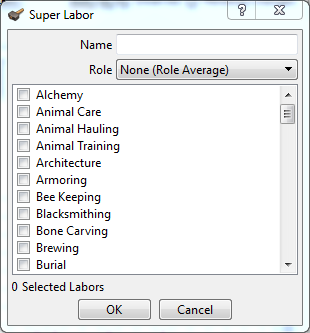
\includegraphics[width=\linewidth]{Sec4Fig18}
  \end{center}
\end{wrapfigure}

Super labors are a recent addition to Dwarf Therapist that allow you to define your own togglable labor
columns out of multiple pre-existing labors. The primary method for creating super labors is to hit
the ``Super Labor'' option on the Customizations dock, which brings you to dialogue displayed at right.
Super labors are in reality a subset of a custom professions---in fact, you can't even name a super labor
something that you have already named a custom profession, or vice versa, as it will cause Dwarf
Therapist to complain. Give the super labor a unique name, associate it with a role (or don't, in which
case a hidden role will be generated and associated with the super labor that uses the average of the
chosen labor's role ratings), and then select the labors that you want to be included in the role. Once
you're satisfied, hit ``OK'' and your new super labor will appear in the Customizations dock as a new
editable (and deletable) item.

A second way to define super labors is to do so using the dwarfwise menu, a procedure that almost exactly
mirrors that of defining a dwarfwise custom profession---click on a dwarf and go to \texttt{Customization
> New super labor from this unit}, and you will be presented with the same dialogue, this time with the
labors that the dwarf currently has enabled, including pending changes, already filled out.

The primary purpose of the super labor is that it allows you to bind together several labors into one
toggle, allowing you to, for instance, unify all of the hauling subtasks, to save on space and sprawl.
Once you have defined a super labor, it will appear in the ``Grid Views'' custom view definition dialogue
as a new item under the ``Super Labors'' menu. A color gradient is used to provide information as to the
number of subtasks enabled: if none are enabled, the box is unfilled; if at least one is enabled, it is
lightly colored; if more, more darkly colored; and if all tasks are enabled, the box is completely filled
out.

In reality, the only thing differenciating a super labor from a custom profession is the lack of an
assigned icon.\footnote{See also \jump{Custom Icons}.} Indeed, custom professions implement super labors
in the background, allowing you to create custom professional multi-labor toggles through the ``Custom
Professions'' item; custom roles also implement them for associated skilled labors, a behavior that can
easily be seen in the ``Roles'' view. Most of the time, you'll want to be implementing custom professions
instead, but you can always create explicit super labors instead you want to cut on cruft. See the
addendum at the end of the next section for an example usage.

\newpage
\subsection{Creating Your Own Grid Views}
\label{sec:Creating Your Own Grid Views}

Copy the Labors NO SPACERS view now, then right click on it and hit ``Edit''. The very first thing you
should do is this:
\begin{figure}[h!]
\centering
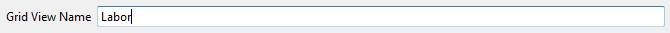
\includegraphics[width=\linewidth]{Sec3Fig15}
\end{figure}

Now if you add that view from the ``Add Views'' drop-down menu and delete the old one:
\fullfigure{Sec3Fig16}

NO SPACERS, banished!

The Grid View window is organized into two columns, sets on the left and
component columns on the right. Set names are not displayed anywhere on-screen, so they're mostly
organizational, but ordering your columns causes the program to automatically apply the set's chosen
coloration to all columns in the set. One column in the game is immutable---your dwarves by default, or
your animals if you've copied the animal view instead. This will always appear on the left edge, and does
not appear in this listing.

Right clicking on a set allows you to either modify it or delete it entirely. Editing the set allows you
to change its name (again, merely organizational) and its coloration---there are a number of predefined
options, but by going to the\texttt{ [...]} option you can choose and use any hex value.\footnote{For
some reason choosing a new color sometimes doesn't change the color of the header. Going through the
menus and just pressing ``OK" again fixes this bug.} Clicking on an empty space in the box creates a new,
empty set for editing. To rearrange the position of a set, simply grab and tug it up or down.

The columns themselves are color-codes to match their sets, but if you edit them you'll be able to
override the base set color and set your own. Right clicking anywhere will also bring up a complete
menu list of possible columns to add to your view. You can also add or remove spacers here---since they
don't serve too great a function, if you don't have the horizontal sceen space for them in a view,
removing them might be extremely helpful.

Now, let's make some modifications to our new and improved ``Labor'' view.

\fullfigure{Sec3Fig17}
\fullfigurecaption{Our Labor View at the beginning of this exercise.}

The first thing we should do is remove alchemy. Assuming you're not using mods, it's not implemented into
the game, and so it has no place in the labor view. Go to Other Jobs, right-click on Alchemy, and hit
Remove.
\vspace{12pt}

There isn't ever a real reason to remove Cleaning as an enabled labor, either---when your dwarves
actually perform that job, it's a blessing---so let's remove that too. This has the benefit of allowing
you to remove all labors from your dwarf with the right click option without removing cleaning as well.
\vspace{12pt}

Though Architecture is held in-game to be an administrative job, despite having a labor assigned to it,
it's really an engineering one. Now that it's left all on its lonesome on the right edge of our screen,
we have an excuse to move it under the engineering banner. I'm placing it between mechanics and pump
operating on the banner.
\vspace{12pt}

Animal care is similarly unimplemented in vanilla at the moment---your animals either heal up, or they
die, and there's nothing you can do about it. So it's safe to send it the same way as alchemy, because
even if some of your dwarves do have skill in it they'll never get to use it.
\vspace{12pt}

Feeding prisoners and the wounded is always a priority job that is or should be enabled on all dwarves by
default, pretty much even the grumbly ones---the rare -20 happiness penalty is minor compared to the cost
of a tantrum spiral. So these two columns are safe to remove, too.
\vspace{12pt}

Now that we've removed useless labors from the display, let's do some organization amongst the tasks that
are left. Farming in particular is a mightily large category, and I often get lost looking for my Weaver
somewhere between my Potash Maker and my Presser, or even start designating the wrong labors on a dwarf!
I have a similar problem with the labors under the ``Crafts'' header. Let's divide these sections between a
few different categories.
\vspace{12pt}

\begin{wrapfigure}{L}{0.05\textwidth}
\vspace{-20pt}
  \begin{center}
    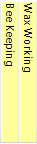
\includegraphics[width=0.045\textwidth]{Sec3Fig19}
  \end{center}
\vspace{-15pt}
\end{wrapfigure}
The first new category I create is beekeeping. Beekeeping is rarely used by players because it's an
extremely labor-intensive and limited form of food production that produces low-value goods and is
heavily bugged. Assuming the bugs with the industry are resolved, it might become more useful in future
versions of the game, but for now we'll relegate it to the sideline.
Beekeeping and Wax Working are both jobs that are only ever used in this industry. The new color of
choice is obvious---yellow.
Open up the customization menu and select the weaker yellow of the two that are available in the menu.
This is still pretty bright, though, so let's weaken the colors a teeny bit further. In the end the color
I used had an RGB value of 255-255-157 (alpha 255), but you can adjust it to your liking.

\begin{wrapfigure}{R}{0.15\textwidth}
  \begin{center}
    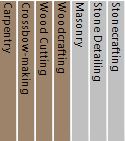
\includegraphics[width=0.15\textwidth]{Sec3Fig20}
  \end{center}
\vspace{-15pt}
\end{wrapfigure}
Woodcrafting is better off alongside its peers in the woodworking column.
\vspace{12pt}

In a similar vein, stonecrafting is better alongside masonry and stone detailing.
\vspace{12pt}

\begin{wrapfigure}{L}{0.11\textwidth}
\vspace{-25pt}
  \begin{center}
    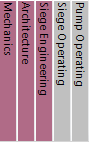
\includegraphics[width=0.11\textwidth]{Sec3Fig21}
  \end{center}
\vspace{-15pt}
\end{wrapfigure}
Pump operating and siege engineering fit a certain theme, so while we're doing all this rearranging let's
give them their own column to the immediate right of their current location. I use the default light grey
color for this column.
\vspace{12pt}

Let's also move Siege Engineering to the right edge of the engineering set, to match Siege Operating
opposite it.
\vspace{12pt}

%\begin{wrapfigure}{R}{0.1\textwidth}
%\vspace{-25pt}
%  \begin{center}
%    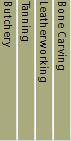
\includegraphics[width=0.1\textwidth]{Sec3Fig22}
%  \end{center}
%\vspace{-15pt}
%\end{wrapfigure}
Butchery, tanning, leatherworking, and bone carving are all components of the meat and leather industry,
and so belong togethor. For this one I used a muddy leathery brown, RGB values 170 170 127.
\vspace{12pt}

Since there's no Other column anymore, let's set the hauling labors to their base white to make more
sense of the skill-less labors.
\vspace{12pt}

Pottery and Glazing work as a pair. For these two I choose a light pink, RGB value 255-225-240.
\vspace{12pt}

Shearing, Spinning, Weaving, Clothesmaking, Dying, and Strand Extraction all have to do with the
clothesmaking industry. For this one I used a downsampled version of one of the base pastel blues, RGB
155-205-255.
\vspace{12pt}

Glassmaking becomes the odd one out of the old crafts column, but folds nicely into jewelry---glass is
just a fancy gem that can also be turned into furniture after all.
\vspace{12pt}

The remaining parts of the large farming cluster were a little trickier to organize. I ended up dividing
it into two tranches with some color variation betwixt them (in color order, default, 218-199-175,
default again, 85-170-127, 193-191-171, 85-170-127 again).
\vspace{12pt}

Then I toned down the medical task colors because the text is really hard to read in that dark a color. I
moved this one down all the way to 140-112-114.
\vspace{12pt}

\begin{figure}
        \centering
        \begin{subfigure}[H!]{0.32\textwidth}
                \centering
                \includegraphics[width=\textwidth]{Sec3Fig23}
        \end{subfigure} ~~~
        \begin{subfigure}[H!]{0.64\textwidth}
                \centering
                \includegraphics[width=\textwidth]{Sec3Fig25}
        \end{subfigure}
\end{figure}

Now some name changes were in order. Why is it Farming (Fields)? Let's just set that to Farming. Why is
it Haul/Push Vehicles? Whenever you are using a vehicle you are pushing it; when you are hauling it to
and from a stockpile it falls under Item Hauling. Let's just change that to Push Vehicles. While it is
true that bowyers are only really crossbow-makers, as they don't make anything else, ``bowery'' is a
much shorter and more elegant name: let's change it to that.
\vspace{12pt}

Finally, glassmaking and bone carving are kind of lopped onto their sets, and siege
operating folds into siege engineering, so I fade those halfway down the coloration scale to
individualize them.\vspace{12pt}

The finished result:
\fullfigure{Sec3Fig26}

It's organized, easy to view, fully color-coded, and nicely streamlined; half an hour well spent.

\addendum{

The ``Super Labors'' feature added since the first version of this guide was published allows us to make
one further, optional refinement to this view: merging all of the hauling sublabors into one. We can use
either the example ``Hauler'' custom profession we defined earlier, or a new, explicit superlabor:

\vspace{5pt}
\includegraphics[width=\linewidth]{Sec3Fig26+}
\vspace{-5pt}

On my 21-inch screen, this was enough to allow me to \emph{finally} use docks without horizontal
scroll bars! There's a full spread on the next page.

}

\subsection{Exporting and Importing Grid Views}
\label{sec:Exporting and Importing Grid Views}

The ability to export and import grid views is very important, given the amount of work that must go
into reproducing a custom view, and both options are available under the ``File'' header in the taskbar.

\newpage
\begin{figure}[h!]
    \vspace*{-2cm}
    \makebox[\linewidth]{
        \includegraphics[width=.85\linewidth]{Sec3Fig29}
    }
\end{figure}
\newpage

\part{Expert Features}
\label{sec:Expert Features}
\section{Filter Scripts}
\label{sec:Filter Scripts}

Dwarf Fortress provides two different, easy-to-use tools for organizing your dwarves. In this section
we'll introduce a third, much more advanced tool for the task: filter scripts. With custom filter scripts
you can filter out those dwarves that you don't need to see right now from those that you do in a much
more powerful, and much more refinable, way than grouping or sorting allows. However, it's also a
challenging thing to do, as it requires that you learn and master the program's syntax for the task;
indeed, if you do not have experience with writing programming code you could very easily become lost
here.

Go to the dedicated Scripting item on the menu bar and hit \texttt{Add New Filter Script} to bring up the
script creation and modification dialogue:

\fullfigure{Sec4Fig1}

As you can see, on the right side there is a fairly detailed demonstration of what filter scripts are
meant to do, and then further down the list we get a list of methods we can use and then several
tabulated references for labor, trait, skill, and attribute ids. You can actually collapse this away to
the side or expand it to take up the whole view by dragging the right edge of the box.

Filter scripts work by generating a boolean test for your dwarves and then iterating through them. Dwarf
Therapist handles looping for you, so your job is simply to write a useful filter: basically, at the end
of the application of your filter to a dwarf, we want to end up with either a ``true`` or ''false''
statement. If the result is false, the dwarf will not be displayed; if it is true, they will be. All of
the commands that you can enter into the script editor are all meant to be called on the ``d'' object, the
abstracted dwarf in question, through the dot operator: \texttt{d.is\_child()}, for instance. The
options are documented fairly well in the lookup box on the right of the box---here's a partial list of
some of the commands available to you:
\vspace{12pt}

\begin{tabular}{l c l}
\textbf{Command} & \textbf{Return} & \textbf{Description}\\
\texttt{is\_child()} & boolean & Returns true if d is a child, else false.\\
\texttt{is\_adult()} & boolean & Returns true if d is an adult, else false.\\
\texttt{is\_animal()} & boolean & Returns true if d is an animal, else false.\\
\texttt{profession()} & string & Returns the basal profession string of a dwarf.\\
\texttt{raw\_profession()} & integer & Returns the raw basal profession ID number of a dwarf.\\
\texttt{custom\_profession\_name()} & string &  Returns the raw custom profession string, NULL if none.\\
\texttt{nice\_name()} & string & Returns the nickname string, NULL if none.\\
\texttt{noble\_position()} & string & Returns comma separated list of noble positions.\\
\texttt{get\_raw\_happiness()} & integer & Returns the raw happiness value of the dwarf.\\
\texttt{attribute(attribute\_id)} & integer & Given the ID number, returns a dwarven attribute value.\\
\texttt{active\_military()} & boolean & Returns true if the dwarf in an active military squad.\\
\texttt{squad\_id()} & integer & Returns squad ID (from 0 by order of formation).\\
\texttt{can\_set\_labors()} & boolean & Returns false if dwarf is a child or baby.\\
\texttt{labor\_enabled(id)} & boolean & Is this labor (by id number) enabled on this dwarf.\\
\texttt{is\_labor\_state\_dirty(id)} & boolean & Returns whether there are pending changes for this skill.\\
\texttt{labor\_rating(id)} & integer & Return's the dwarf's skill in a labor.\\
\texttt{trait(trait\_id)} & integer & Returns raw trait value by ID number.\\
\texttt{total\_assigned\_labors()} & integer & Returns the total number of assigned labors for this dwarf.\\
\multicolumn{3}{r}{Optionally takes a boolean value: if set to false, does not include hauling labors.}\\
\multicolumn{3}{l}{\texttt{skill\_level(int skill\_id, bool raw, bool precise)}}\\
\multicolumn{3}{r}{Returns a floating point value, or ``float".}\\
\multicolumn{3}{r}{Raw uses the uncapped skill level, precise returns a decimal skill level.}\\
\multicolumn{3}{l}{\texttt{has\_health\_issue(category, index)}\quad boolean}\\
\multicolumn{3}{r}{Returns the health status of this dwarf.}\\
\multicolumn{3}{r}{The optional index item allows you to check for a specific condition.}\\
\end{tabular}
\vspace{12pt}

\noindent In addition to being able to call on attributes through \texttt{attribute()}, you can also call
on them directly by name:
\begin{multicols}{3}

\begin{verbatim}
int strength()
int agility()
int toughness()
int endurance()
int recuperation()
int disease_resistance()
int analytical_ability()
int focus()
int willpower()
int creativity()
int intuition()
int patience()
int memory()
int linguistic_ability()
int spatial_sense()
int musicality()
int kinesthetic_sense()
int empathy()
int social_awareness()
\end{verbatim}
\end{multicols}

As for logical construction, Dwarf Therapist uses standard boolean operation notation. \texttt{||} stands
for OR, and two statements linked in such a way will return true if either or both are true.
\texttt{\&\&} means AND, and will only return true if \emph{both} statements are true. Statements based
around a \texttt{==} operator will be evaluated for equivalency, and will return true if they are, and
false if they are not. Statements surrounded by \texttt{()} operators will be evaluated ahead in PEMDAS
order, much like they are in algebra. Finally, adding a \texttt{!} before a boolean statement negates
it---false becomes true and true becomes false. Integers can be compared with \texttt{<} and \texttt{>}
operators as well as the \texttt{==} one. Strings must be surrounded in double quotes, \texttt{"Like
This"}.

\subsection{Writing Complex Scripts}
\label{sec:Writing Complex Scripts}

%\legacy{All of the scripts defined in this section are now provided as program defaults.}

Now that we have the basic syntax down, let's use filtering to solve a non-trivial problem. Whenever a
large migrant waves arrive at a fortress, or even a small one in a lot of cases, what happens is that you
pick the best of the bunch and set them to work immediately, and get the rest of the wave doing generic
tasks that are plentiful and easy to designate---hauling things, getting rid of loose stone, building
walls and other constructions, smoothing and engraving the fortress living spaces, and so forth.
Integrating a new wave into your fortress is a slow but steady process, involving picking off individual
dwarves for tasks you need done on a longer term one by one. Some will become jewelers, some will start
operating furnaces, some will build parts for your pump stack, some will be enlisted in the military---and some will remain plain old haulers.

In  \jump{Using Roles} we discussed combining groups, sorts, and roles to find ideal
dwarves for a particular task within a group, but we were hamstrung by the limitations of a group:
there's no easy way to group ``gainfully employed" dwarves committed to their tasks apart from
``part-time" ones that aren't. Your options were to make do with grouping them into migrant waves, which
doesn't usually end with you selecting the best available dwarf in the \emph{fortress} for the task, or
not grouping them at all, which requires you browse through dwarves that are already working on something
and risks switching the tasks of a dwarf you'd designated for a new role earlier (a problem discussed in
\jump{Assigning Nicknames}). We're going to neatly resolve this little problem with a
script we're going to write.

\fullfigure{Sec4Fig2}
\fullfigurecaption{In my fort I just started funneling my dwarves into tower fortress building duty.}

Whenever you write a script the first question you've got to ask is, "what are the characteristics of a
dwarf that I want`` (if you're writing an \emph{inclusive} script), or ''what are the characteristics of a
dwarf that I \emph{don't} want" (if you're writing an \emph{exclusive} one). In this case we're writing
an inclusive filter meant to root out migrant dwarves that are available for full-time assignment to
useful tasks. If we think about what this implies, we can come up with a number of ``characteristics'' for
such dwarves (in order of complexity):

\begin{enumerate}
\item They have all hauling labors enabled. This is one of the most apparent indicators of a
``working-class" dwarf, but it's nowhere near exclusive.

\item They don't have a nickname. Assuming you follow the advice given in
\jump{Assigning Nicknames}, nicked dwarves have already been dedicated to something.

\item They have the masonry and/or stone detailing labors enabled, but are never above ``adequate'' skill
in the former (since actually building stone blocks is assigned to dedicated masons), and never above
``competent`` in the latter (I consider ``skilled'' the breaking point for when an engraver is actually worth
his salt, and should be taken out of the working-class pool).

\item They are never enlisted in the military (at least, not permanently). At least in \emph{my}
fortress, once a crossbowdwarf, always a crossbowdwarf slash hunter.

\item They never have certain ``key'' labors that are handled by dedicated dwarves enabled (mining,
carpentry, woodcutting, stonecrafting, cooking, brewing, any of the metalsmithing tasks, either of the
jewelry tasks, and clothesmaking). The precise composition of this list may vary somewhat for you, but
most players learn to dedicate certain tasks to certain dwarves to maximize results very quickly.

\item If they are skilled in certain useless or niche tasks (animal caretaking, small animal dissection,
fish dissection, bee keeping, wax working, soap making) they have those tasks enabled. No one creates
extra work for themselves by actually turning these \emph{off}, at least not until you want this dwarf
doing something for you.

\end{enumerate}

Now this is a pretty extensive list of characteristics common to our ``working class'' dwarves, and most
of them require we do some thinking through as they're not immediately obvious.
Hopefully this set of conditions both accurate and precise enough to work. To write such a complex
script, let's break it down into individual steps.
\vspace{12pt}

\textbf{All Hauling Labors are Enabled}\\
This one's pretty annoying; we have to form an AND string out of \texttt{labor\_enabled() == true}
calls. However, a smarter solution that requires less work, both by the program and by us, would be to
call\\\texttt{total\_assigned\_labors()} twice, once asking for labors with hauling included, once
without, and subtract to see if we get the number we want. The behavior of this command is actually
non-trivial: not only regular hauling but the two medical chores are folded in as well, and this isn't
said anywhere in the documentation (well, now it is). That means that our magic number is 11:

\begin{verbatim}
d.total_assigned_labors(true)-d.total_assigned_labors(false) == 11
\end{verbatim}

%And if you plug that into your script editor and hit ``Test Script'' this is what you'll see:
%
%\begin{figure}[h!]
%\centering
%\includegraphics[scale=.91]{Sec4Fig3}
%\end{figure}

This script alone reduced my fortress from 70 to 38 candidates! In fact, the capacity to filter your
dwarves by whether or not they have hauling enabled is actually extremely useful on its own, and there's
no other way to do this kind of thing in the program. So let's keep it! Give the script a name and hit
``Save''. We can actually also write a quick Hauling \emph{Disabled} script, too, now:
\begin{verbatim}
d.total_assigned_labors(true)-d.total_assigned_labors(false) <= 10
\end{verbatim}

\textbf{If Masonry or Stone Detailing are Enabled, they are at a low Skill Level}

Masonry is labor number 13 on the list, and stone detailing is number 12. We write separate tests, one
asking if the dwarf has masonry enabled but is below skill level 3 in it, and one asking if they have
stone detailing enabled but are below skill level 4 in it. We then link these with an OR. This is what
the complete condition test looks like:
\begin{verbatim}
(((d.labor_enabled(13) == true &&  d.labor_rating(13) < 3) ||
d.labor_enabled(13) == false)|| 
((d.labor_enabled(12) == true &&  d.labor_rating(12) < 4) ||
d.labor_enabled(12) == false))
\end{verbatim}

Then we create a new ``Available for Work" script, and within it link the two statements we've written so
far with an AND. So far, so good: on to the next condition.
\vspace{12pt}

\textbf{They are Never Enlisted in the Military}

This one's elementary, just test if the dwarf is in an active military squad and slap a \texttt{!} on it:
\begin{verbatim}
!d.active_military()
\end{verbatim}

This isn't that useful as a standalone filter because there's a group for it. Next!
\vspace{12pt}

\textbf{They Never have a Nickname}

This is fairly simple, though the call is somewhat confusingly named:

\begin{verbatim}
d.nice_name()==""
\end{verbatim}

\vspace{12pt}

\textbf{They Never have Certain Key Labors Enabled}

This one involves a lot of table lookup:
\begin{multicols}{3}
\begin{verbatim}
!d.labor_enabled(47) &&
!d.labor_enabled(48) &&
!d.labor_enabled(29) &&
!d.labor_enabled(11) &&
!d.labor_enabled(33) &&
!d.labor_enabled(38) &&
!d.labor_enabled(45) &&
!d.labor_enabled(50) &&
!d.labor_enabled(51) &&
!d.labor_enabled(49) &&
!d.labor_enabled(00) &&
!d.labor_enabled(53) &&
!d.labor_enabled(46)
\end{verbatim}
\end{multicols}

If you drop the negations and use OR statements, you pretty much get a list of key dwarves in your
fortress: I call it ``Key Dwarves''. It's very useful for getting rid of new migrants who happen to be
novices in skills that are dedicated to, say, my legendary woodcutter, so that they don't take up our
only axe to cut down a tree a minute while the \emph{real} lumberjack sits around doing nothing in
particular.
\vspace{12pt}

\textbf{Niche and Useless Labors Still On}

This is pretty much an inversion of the above: there we had key labors off, here we have useless ones on,
but since it's conditional (and we don't have if statements available to us) it's a little more complex.
It's important to note that dabbling is considered skill zero---\emph{completely} unskilled is considered
skill level -1. So it's time for some more table lookup:
\begin{verbatim}
((d.labor_rating(16) > 0 && d.labor_enabled(16)) || (d.labor_rating(16) <= 0)) &&
((d.labor_rating(43) > 0 && d.labor_enabled(43)) || (d.labor_rating(43) <= 0)) &&
((d.labor_rating(26) > 0 && d.labor_enabled(26)) || (d.labor_rating(26) <= 0)) &&
((d.labor_rating(72) > 0 && d.labor_enabled(72)) || (d.labor_rating(72) <= 0)) &&
((d.labor_rating(71) > 0 && d.labor_enabled(71)) || (d.labor_rating(71) <= 0))
\end{verbatim}

Those are all our conditions; behold, the completed script!
\begin{verbatim}
// hauling test
(d.total_assigned_labors(true) - d.total_assigned_labors(false) == 11) && 
// masonry and stone detailing test
(((d.labor_enabled(13) == true &&  d.labor_rating(13) < 3) ||
d.labor_enabled(13) == false)  ||  ((d.labor_enabled(12) == true && 
d.labor_rating(12) < 4)  || d.labor_enabled(12) == false)) &&
// nickname test
(d.nice_name == "") &&
// military duty test
!d.active_military() &&
// key dwarf test
(!d.labor_enabled(47) && !d.labor_enabled(48) && !d.labor_enabled(29)
&& !d.labor_enabled(11) && !d.labor_enabled(33) && !d.labor_enabled(38)
&& !d.labor_enabled(45) && !d.labor_enabled(50) && !d.labor_enabled(51)
&& !d.labor_enabled(49) && !d.labor_enabled(00) && !d.labor_enabled(53)
&& !d.labor_enabled(46)) &&
// useless labors test
((d.labor_rating(16) > 0 && d.labor_enabled(16)) || d.labor_rating(16) <= 0)
&& // Animal Tr.
((d.labor_rating(43) > 0 && d.labor_enabled(43)) || d.labor_rating(43) <= 0)
&& // Fish Diss.
((d.labor_rating(26) > 0 && d.labor_enabled(26)) || d.labor_rating(26) <= 0)
&& // Animal Diss.
((d.labor_rating(72) > 0 && d.labor_enabled(72)) || d.labor_rating(72) <= 0)
\end{verbatim}

\newpage
\begin{wrapfigure}{R}{0.2\textwidth}
\vspace{-5pt}
  \begin{center}
    \includegraphics[width=0.2\textwidth]{Sec4Fig4}
  \end{center}
\vspace{-15pt}
\end{wrapfigure}
Over the course of composing this script we actually wrote three other useful scripts, which I think is a
\emph{pretty good} demonstration of their utility. Unfortunately Dwarf
Therapist does not provide any facilities for exporting or importing filter scripts, which is a
unfortunate, because filter scripts get very complicated and having to copy other people's scripts
manually is very annoying, as even a single error or typo will likely invalidate the entire thing.
If you like the scripts that were provided here, just copy-paste them into your program!

\subsection{Running Filter Scripts}
\label{sec:Running Filter Scripts}
\begin{wrapfigure}{R}{0.5\textwidth}
  \begin{center}
  \vspace{-20pt}
    \includegraphics[width=0.5\textwidth]{Sec4Fig4+}
  \vspace{-20pt}
  \end{center}
\end{wrapfigure}

Once you have a complete filter script running it is a matter of navigating to the ``Add Filter'' item
on the indicator bar, going to the drop-down menu, and activating your script. Crucially, Dwarf
Therapist allows you to run multiple filter scripts simultaneously, allowing a useful degree of finesse
in your filtering. The sidebar by the drop-down menu will display the number of scripts you have active;
clicking on it removes all active filters and resets the screen. If multiple scripts are active you can
use the drop-down menu to remove them individually as well. This allows you to easily check
how many of your key dwarves have hauling enabled, for instance, and to perform other such flexible
tasks.

Furthermore, by typing into the ``Filter Dwarves'' text field, you can search for your dwarves by name and by item preference, or through an amalgamation of the two. This is the easiest way to find an individual dwarf by name, as briefly mentioned in the introductory section \jump{Group By and Filters}, and allows you to search dwarves by preference without having to rely on the ``Preferences'' dock. Indeed, all of the docks that include a search capacity---the ``Thoughts'', ``Preferences'', and ``Health Legend'', specifically---execute their searches through a filter, and this filter will be applied through, and removable by, the ``Active Filters'' button. This dynamic filtering capacity is a feature currently under development, and health and preference filters will be added by future version of Dwarf Therapist.

\subsection{Exporting and Importing Filter Scripts}
\label{sec:Exporting and Importing Filter Scripts}

Unfortunately Dwarf Therapist does not currently provide an interface for exporting or importing filter
scripts beyond the ability to copy paste the contents of the script editing pane. Such a feature is
planned for a future version of the utility.

\newpage
\section{Optimization Plans}
\label{sec:Optimization Plans}

%\legacy{The optimization plan created here is now included as a test plan in the default installation.}

Optimization plans are a (somewhat complicated) way to automate the labor assignment process that we've
so far been doing manually. To access it, go to \texttt{Optimization > New Optimization Plan}, which
should bring up a screen similar to the following one:

\fullfigure{Sec4Fig5}

This isn't the easiest of screens to piece apart, so let's look at what each option is meant to do first.
It isn't immediately apparent, but the labor optimizer works by assigning jobs in a ratio-wise manner.
The two numbers in the top right corner tell you how many dwarves are being considered, and how many of
those dwarves will have their labors specialized in the current assignment scheme. If you do not select
any dwarves the optimizer will work with all available dwarves, but if you select a dwarf (by clicking on
their name) or multiple dwarves (by dragging the mouse down dwarves in a column, or by clicking on
the first dwarf and shift-clicking on the last one) it will constrain itself to those
dwarves.\footnote{You can also select all with the \texttt{Ctrl + A} hotkey.} You can use filters to
only display those dwarves that you want to be optimized---I recommend using the ``Available for Work''
filter we just wrote in the last section, \jump{Writing Complex Scripts}.

Let's use the optimizer for a simple task---say, assigning  (role-optimized) dedicated wood burner and
furnace operator from betwixt a few dwarves. Open a new optimization plan again. Set ``max jobs per dwarf''
to 1. This obviously restricts the maximum number of jobs a dwarf can be assigned to just one job, which
makes sense given what we're trying to do. Disable ``auto-assign haulers''---this is a more advanced
feature that we'll talk about in a moment. Now set ``Percent Total Jobs'' to 100. This number tells the
optimizer that we want all of the jobs that these dwarves can be assigned to be assigned in our
optimization scheme.

Roll your mouse over the empty white space and right click to bring up a menu of labors, and select first
``Wood Burning`` and second ``Smelting'' from the list. You can add any number of labors to the list in
this manner, and you can easily delete any labors you've already added by right clicking and hitting
``Remove Selected''.

\begin{figure}[h!]
\centering
\includegraphics[scale=1]{Sec4Fig7}
\end{figure}

The first thing listed here is the job---the labor title that you've select. The next item is the role by
which the optimizer is examining your dwarves' fitness: the one assigned to the job at hand by default.
It's possible to use custom roles here. For the task at hand, however, leave this as is. Priority,
meanwhile, changes the weight with which role fitness is considered, and so shifts overlaps in favor of
the higher-priority labor. The ratio changes the amount of dwarves that will be
assigned this labor by the optimizer relative to the set. For any particular job the ratio is
divided by the sum of the ratios, giving you the percentage of jobs that will be assigned under that
labor, which when multiplied by the number of jobs to be assigned gives you the last column---the worker
count.

We don't have to actually change anything here: everything seems to be in order, with one job going out
for wood burning and one for furnace operating. Let's name our plan ``Test Plan'' and save it. This allows
us to edit or remove our new optimization plan from its associated taskbar item, and you can test your
plan in-view using the ``Test Optimize'' button. Properly applying your designation, however,
requires a new item that appears on your main menu bar---the optimization button.

\fullfigure{Sec4Fig8}

This button will not appear when you don't have any optimization plans saved. When you have multiple
optimization plans, a button appears besides it that lets you drop down a menu to select which script is
the active one---this also applies the script in question, saving you a mouse click.

Now selecting any number (or, as earlier, selecting none and therefore all) of dwarves and
hitting Optimize will cleave them in two, between the wood burners and the smelters. If the number of
dwarves selected is odd you will get an uneven number of job divisions---in this case three furnace
operators but only two wood burners.

\fullfigure{Sec4Fig10}

Now let's add a fold of complexity to our plan by including hauling as well. To edit an optimization
plan, go to ``Optimizer`` on the taskbar and select the plan from the ``Edit Optimization Plan'' menu. This
time let's turn auto-assign haulers on and set it to 50 percent: likewise, set the total jobs percentage
to 50 as well. Now hit ``Test Optimize" at the bottom of the window to see what effect this plan has on
our dwarves (I deliberately avoided doing this earlier to showcase predefined usage and the changes to
the menu bar). As you might have guessed this cleaves our dwarves in two: a quarter each are assigned
dedicated wood burning or furnace operating, and the remaining half are made haulers, with their other
labors disabled. A note that needs to be made: optimization plans will obviously only work properly if
roles are tuned to the default skill rank setting we discussed in \jump{Roles}.

\fullfigure{Sec4Fig11}

From our little group of five dwarves this results in one wood burner, one furnace operator, and three
haulers. Once again because five is indivisible by two the division is uneven, with more haulers being
assigned than workers.  This is the reason that the numbers that the dialogue gives us are approximate -
if the numbers don't fold there will inevitably be some fudging on the corners.

Let's dig a little deeper. Set the maximum number of jobs a dwarf can have to 2 this time, and test the
script again to see what effect this has:
\fullfigure{Sec4Fig12}

Unless you're particularly insightful, it's probably not immediately apparent what's going on here---why
is only one dwarf hauling anything? So far we've generated three optimization scenarios; now let's use
them to get a better understanding of how the labor optimizer works.

The percent total jobs parameter is a cap on how many jobs can be assigned, out of how many total
possible jobs there are. In the first example this number was set to 100, so the labor optimizer could
give every dwarf a job to do. Since the max jobs per dwarf parameter was set to 1, every dwarf could only
get one job total. Since we have two labors of equal priority under consideration, this means that half
of the dwarves will recieve the wood burning task, and nothing else, and half would recieve the furnace
operating task, and nothing else.

In the second example, we reduced the cap to fifty percent, and kept the number of jobs per dwarf at 1.
This means that \emph{fifty} percent of dwarves will be assigned \emph{one} job. Indeed, ignoring some
fudging that the program had to do, again because five is not divisible by two, half of half of the
dwarves recieved the wood burning labor and half of half of them received the furnace operating labor.

How did the program behave in the last example? This time the percent labor cap (let's just call it the
labor cap from now on) was still set to 50, but the maximum number of allowed jobs (let's just call it
the job cap from now on) was set to 2. We still have two labors, but now we also have two ``spaces'' for
them to be assigned to. In the resulting configuration \emph{fifty} percent of dwarves are assigned wood
burning, but then \emph{another} fifty percent are \emph{independently} assigned furnace operating.
Logically, because the labor optimizer has been allowed to assign jobs twice instead of only once,
dwarves that are fitter than the group average at both wood burning \emph{and} furnace operating will be
assigned both jobs. The labor cap no longer regulates how many jobs the two labors together can be
assigned, but how many times they can appear individually. Under the single-job scheme, two labors had to
contend against one another under the fifty percent job cap, and so each labor could only be turned on 25
percent of the time; under the two-jobs scheme this is no longer the case, and so each labor could be
turned on a full 50 percent of the time.

In another form, the number of labors that will be turned on will thus be given by the following equation
(note that you have to divide the labor cap by a hundred because it is in percentage form):
\begin{displaymath}
jobs\:cap \times number\:of\:dwarves \times  \frac{labor\:cap}{100} = number\:of\:labors\:to\:be\:assigned
\end{displaymath}

And the number of assignments for each individual labor, which is dependent on the ratio, is as follows:
\begin{displaymath}
number\:of\:labors\:to\:be\:assigned \times \frac{that\:labor's\:ratio}{sum\:of\:labor\:ratios}
\end{displaymath}

Let's take this to its logical conclusion: what would happen if we kept jobs cap at 2, but raised the
labor cap to 100 percent? Logically that would mean that every instance of that labor will be assigned -
and a quick test confirms that, indeed, that is the case:
\fullfigure{Sec4Fig13}

What about the funkiness with the assignment of hauling in example three? If you were following along
with the examples I was giving, and didn't check the tooltip text on the Hauler Percent box in the
dialogue, you might have (wrongly) concluded based on the parameter's behavior in examples one and two
that the optimizer assigns hauling to a certain percentage of the total dwarves under consideration. That
is not the case: rather, that percentage is a bit of dwarf-wise post-processing optimization based on how
many labors that dwarf already has assigned.

Basically, the optimizer assigns labors, then goes down the list and asks each dwarf how many labors they
have assigned: one? Two? None? It then compares this to the ``Hauler Percent" value (hauler threshold
from now on), and if the dwarf has fewer than that percent of the maximum number of labors assigned, then
they are assigned hauling tasks. In the example above every dwarf has both labors enabled, and so
obviously no dwarf falls under the fifty percent threshold---and no dwarf is assigned hauling. In example
two three of our dwarves don't have anything assigned post-processing, so they obviously get hauling
booted onto them.

Example three actually demonstrates an optimization behavior that's important to know: that the hauling
threshold is strict. Dwarves one and five both have one labor assigned, which is half of two, the number
of labors they \emph{could} have assigned. In percent form one over two is fifty percent: on the border
of our threshold, but not below it. To get the behavior we want, increase the threshold to 100 percent:
\begin{figure}[h!]
\centering
\includegraphics[width=\linewidth]{Sec4Fig14}
\end{figure}

The number required is 100 percent, and not 51 percent, because of the program's behavior.

There's just one more thing to be said% before we move on to application.
: you can exclude various groupings from optimization right from the dialogue by unchecking their
associated boxes:
\begin{figure}[h!] \centering \includegraphics[scale=1]{Sec4Fig6}
\end{figure}

Excluding hospitalized dwarves is important if you want the jobs done now, but isn't necessary if no one
(or no one freely available to work \emph{and} under consideration) is injured, and may be
counterproductive if on the flip side a significant number of your dwarves have sustained recoverable
wounds. Excluding nobles is a poorly optimized solution because while assigned nobles work as normal,
royal nobles will not have much of a work ethic regardless of what tasks you assign to them---you usually
won't be considering nobles regardless, so not excluding them is a safe bet. There is some overlap
between ``active military'' and ``squads'': dwarves are considered to be on active duty when they are on
call, correspondingly appearing by their military position in-game---but to get that far they obviously
have to be assigned to a squad first. Excluding squads is important when your military is fully
professional, but of dubious use when you have a attack-that-thing-now dwarven militia that you never
disbanded.

As it turns out, dwarf number five in our examples above is actually a noble---I just haven't been
excluding him in the optimization process. Doing so results in exactly the sort of behavior you would
expect---he's ignored---and has the nice side effect of tidying up our ``five divided by two" problem.
\fullfigure{Sec4Fig15}

\subsection{Using Optimization Plans}
\label{Using Optimization Plans}

See \jump{Putting it all Together}.

% 
% Simple optimization plans are easy to write and an extremely handy time-saving tool when applied in scenarios like the one described above---when you are looking to start off an industry. In these cases it's handy to have a preset labor optimization plan that's preloaded with the jobs needed in the industry, as well as, for the purposes of standardizing your industry-starting practices, a number in mind for the amount of dwarves you want optimized. I call such optimization plans ``Industry Starter Plans'', and we'll write one as an exercise here.
% 
% One thing that you're always going to have to eventually do is invest in a textile industry, preferably sooner rather then later so as to avoid naked dwarves tantruming all over your dining hall.

\subsection{Exporting and Importing Optimization Plans}
\label{sec:Exporting and Importing Optimization Plans}

Like most of the configurable utilities packaged into Dwarf Therapist, optimization plans can be exported and made available for others to use, or imported and made available for use in your program. This feature is only available from the options bar on the optimization plan editing menu, as it doesn't
appear in the Optimization taskbar item.

\fullfigure{Sec4Fig17}

\newpage
\addendum{
\section{Addendum: Memory Tools}
\label{sec:Scanning Memory}
If you click on the ``Scan Memory'' item in the File menu you will be brought to the Dwarf Therapist memory
scanning utility:
\vspace{12pt}

\includegraphics[width=\textwidth]{Sec4FigExtra}

\center{The result of a brute-force search for the string ``hauling''.}

\vspace{6pt}

% \begin{wrapfigure}{R}{0.28\textwidth}
% \vspace{-20pt}
%   \begin{center}
%     \includegraphics[width=0.28\textwidth]{Sec4FigExtra3}
%   \end{center}
% \vspace{-15pt}
% \end{wrapfigure}

\begin{flushleft}
\textbf{This will not be covered in this guide}. Dwarf Fortress memory mapping and modification is not
for the faint of heart, and is used for two things: finding the RAM values for things necessary to get
complex utilities and mods working (like, say, Dwarf Therapist), and cheating the game by changing them.
The first is way out of the scope of this guide, and for the second there are much more elegant tools
available: as labor management has been given a GUI by the community, so to has memory access and
modification. I'm also not going to pretend I fully understand how the tool even \emph{works}.

Additionally, if you right click on a dwarf's name and scroll to ``Memory Tools'' you will see that there
are some memory options available for individual dwarves as well. You can ``Dump Memory" to open the
memory matrix associated with that dwarf tabulated in a text box by the program. ``Dump Memory to File"
will also read the dwarf's memory values into a chart, but will save it to a \texttt{TXT} file in the
Dwarf Therapist log subfolder. Finally, you can ``Copy Address to Clipboard" to copy that dwarf's memory
location to your clipboard. This function may be useful if you're interested in modding your dwarves
in-game, but once again it's not something the average user would need.
\end{flushleft}
}

\newpage

\section{Putting it all Together}
\label{sec:Putting it all Together}

\fullfigure{Sec5Fig1}

We have now individually covered all of the features available to you in Dwarf Therapist, and so we are
ready to put togethor everything we have learned so far and employ towards solving a particularly
complex task: military recruitment.

One of the most time-consuming and complex tasks in Dwarf Fortress is the creation, assignment, and
management of military dwarves and military squads. Our goal in this section of the guide is to put
together everything that we've learned up to now and apply it to this thorny problem, starting with
streamlining the process for conscripting dwarves into our squads.

The first thing we want to do is think about what kind of a view we will need for this task, as the
default military view is far too comprehensive for the purposes of simple recruitment. Instead we are
going to build our own, specialized view for the task. Let's begin by looking at how squads in Dwarf
Fortress are or ought to be structured. You can have up to ten dwarves per squad, with a squad leader,
subordinate to your assigned militia commander noble, and up to nine other dwarves. You can give each
dwarf in a squad an individual uniform, but it's easiest and most logical to make them uniform: every
dwarf in a squad is equipped with the same weapons and approximately the same kit, uniform availability
depending. Clearly our squad leader should differ from his compatriots: he needs to be not only an
excellent fighter, but also an excellent teacher and leader, so we are going to need roles for both
individual fighting dwarves, and slightly more demanding ones for their officers.

Dwarves can use any weapon that they can wield out of a certain large set of them---you can see the full
list of wieldables, and whether or not individual dwarves can wield them, in the ``Weapons'' view or in
the ``Military'' view. However, we are not going to concern ourselves with most of the items on this
list, since they either cannot be produced domestically or cannot be wielded at all, and since dwarves
will never come to your fortress with experience in weapons, like whips, which are not
sufficiently ``dwarvish''. Thus our list of possible squad weapons is: battle axes, crossbows, maces,
short swords, spears, picks, and war hammers. To be comprehensive, then, we will need to define a custom
role for wielders of each of these weapons, as well as a parallel ones for their officers. Additionally
we can define melee-generalist ``meleedwarf'' and ``lead meleedwarf'' roles, for squads with dwarves
meant to equip whichever weapon they are most skilled in already, to better take advantage of
pre-existing skill rank. That brings us to a total of sixteen custom roles, split between our regular
conscripts and our officers. \emph{However}, Dwarf Therapist ships with specific militiadwarf roles,
excepting pickdwarf, already defined---so we have only the various officer dwarf roles, and the
meleedwarf and pickdwarf roles, to define. Let's begin by writing these roles.

\step{1}
What's the difference between a meleedwarf and an axedwarf, or a hammerdwarf, or so on? None, except that
he is excepted to be versed in any one weapon, as opposed to a specific one of your choosing. So to
generate a meleedwarf custom role, open up the Custom Role definition window with \texttt{Roles > New
Custom Role}, and copy in any meleedwarf role---axedwarf is closest. Add to this role all of the
domestic melee weapon skills and domestic weapon preferences not already listed, and save the role.

The process for creating a pickdwarf role mirrors that for creating the meeledwarf one, except that
instead of importing all of the remaining weapons we instead kick out whatever weapon is in the role we
copied, and add the mining skill and pickaxe preference.\footnote{Picks are not predefined because they
are hardly ever used for combat, being meant for mining and all that---they even level with the
Mining skill, instead of a dedicated combat skill. Not a very sexy weapon, but very effective in a
pinch, I hear.}

What makes for a good dwarven officer? Open up the role definition window again, and this time copy in
your new meleedwarf role. Add to it the attributes (linguistic ability and social awareness) and skills
(teacher) associated with the ``Teacher'' role, and save (you can also add some traits, like ``bravery''
and somesuch, if you'd like). For the rest of the officer roles, just repeat this process. Tedious, but
not difficult---if you don't want to bother, I include a packaged export of everything we create here at
the end of this section.

\step{2}
Now that we have all of the roles we want to use defined and ready, let's create a part of the
view in which we can use them. Open up the Grid View dock (\texttt{Windows > Docks > Grid Views}) and
hit ``Add a New Grid View''. Name your view something appropriate---I called mine ``Recruitment''---and
let's add what we have so far.

\fullfigure{Sec5Fig2}

Note that the ``Pickdwarf'' columns are labor toggles. If you inspect them you'll notice that, in a
behavior described earlier in the addendum to \jump{Using Roles---The View Method}, roles with skilled
labors associated with them (in this case, mining) will be togglable for those labors.

\step{3}
Within Dwarf Fortress only active-duty soldiers are assigned their military professions---when they are
off-duty they are given their civilian professional names instead. This is fine when we have a part-time
militia, but less helpful when we are trying to raise and train a professional military command. So let's
write custom professions we can assign to fix this problem for us. No need to define lead dwarf
professions, either---their status as assigned nobles tells all.

It's easiest to do this out of the ``Customizations'' dock. The labors I assign to my dwarves are hauling
for everyone, pump operating for all meleedwarves (pumps that don't pump anything are a great physical
training regimen), hunting for all marksdwarves, mining for all pickdwarves, and wood cutting for all
axedwarves.

%\newpage
%\begin{figure}[h!]
%\centering
%\includegraphics[width=.4\linewidth]{Sec5Fig3}
%\end{figure}


\step{4}
Let's now add these professions to our view! And while we're at it, let's add a set of columns for
experience in the raw military skillsets we're using.

\fullfigure{Sec5Fig5}

\newpage
\step{5}
We now have our custom recruitment view in place, as well as a liturgy of appropriate new super-labors
and professions in the customizations dock. The filter script we're going to use to weed fortress
regulars from conscription is obvious---it's the availability script we wrote as an example in
\jump{Filter Scripts}. This leaves us with only one last thing to write: our optimization plan, or
perhaps plans.

An optimization plan that optimizes just one squad of dwarves isn't strictly necessary, since you can
sort the dwarves, assign them their labors, and then assign them the profession. Optimization plans can't
assign professions, only labors, so you're not saving on much work with a single-squad plan. Instead we
want to write a ``Military Starter'' optimization plan, similar to the ``Industry Starter'' plans that
provide the bulk of this feature's utility. Usually, when I decide it's time to start a professional
military, I start off with two squads: one of marksdwarves, and one with some sort of melee weapon.
The usefulness of an optimization plan in this case is that it allows us to assign two squads of roughly
equal parity. If we have a dwarf under consideration who is in the selection percentile for two
different squads, then if you assign him manually, the squad he goes to will be a matter of which squad
you assigned first. If you have an optimization plan, on the other hand, he'll go where he is needed
most.

To do this, assign ``Hunting'' and ``Pump Operating'', the two labors which are unique to marksdwarves and militiadwarves, respectively, in equal amounts in your plan, and save.

\step{6}
There is one last thing we need to write: a simple filter script that only displays dwarves with
pending changes, or ``dirty cells''. You'll see in a little bit why this is necessary. The filter is
simple in concept, but large in size, since it requires that we call \texttt{d.is\_labor\_state\_dirty()}
on all possible labors---all 73 of them!

%\begin{figure}[h!]
%\centering
%\includegraphics[width=.5\linewidth]{Sec5Fig6}
%\end{figure}

We now have all the custom definitions we need to conscript our dwarves! Now let's walk through the
process of actually assigning them.

\step{1} Filter your dwarves down to those that are available for assignment, using the availability
script we wrote in \jump{Writing Complex Scripts}.

\step{2} Sort the dwarves by officer fitness, first in marksdwarvemanship and second in
meleedwarvemanship. Take note of the names of those dwarves that appear at the top of the list. Within
Dwarf Fortress, go to the ``Nobles'' screen (\texttt{N}) and make the fittest dwarf you have for each
officer role a militia captain, sheriff, captain of the guard, or militia commander, whichever is
appropriate. Since this is only the start of our budding military, it's probably best to make the head
meleedwarf the militia commander, and the head marksdwarf the captain of the guard or
sherrif.\footnote{Dwarves with crossbows elect to dole out physical punishment by beating dwarves with
their crossbows, hence why they make good guards. Assuming you make your crossbows out of wood, this
will have \emph{much} less gruesome results then, say, hacking at the poor dwarf with a sword!} I also
recommend you name the squads something functional, so you can distinguish between them at-a-glace
in-game: ``Fortress Guards'' and ``First Meleedwarves'', for instance.

\step{3} Re-read dwarves from Dwarf Fortress, so that Dwarf Therapist can see the new squads. Filter them
again down to those available for assignment.

\step{3} Select all dwarves displayed using \texttt{Ctrl + A} then go to the plan editor again. We want to optimize twenty dwarf, but have available some number of them, save, 80. With some quick math, it becomes apparent that we want to optimize 25 percent of our dwarves---so enter that value into the Percent Total Jobs textbox, and save. Now run the plan!

\addendum{Numerical optimization, a feature planned for future releases, will automate this procedure.}

\step{4} Now add the ``Pending Changes'' filter we defined in step six to the active filters, to remove
those dwarves that escaped military assignment (this round) from the view.

\step{7} Click on each dwarf with pending changes and assign them, from the dwarfwise menu, the proper
military profession (and with it, the proper labors), and the proper squad. Remember---since we've
already assigned the officers separately, we only have the remaining 18 dwarves to go through.

\step{8} Hit commit changes and admire your new dwarven military squads! The fun's not over, though,
since you now have to go to the Dwarf Fortress military screen (\texttt{M}) and start assigning
uniforms, schedules, and so on.

\vspace{12pt}
And there you have it!

\newpage
\part{Appendix}

\section{Hotkeys}
\label{sec:Hotkeys}

Although the main functions that you'll be performing with the program have hotkeys, overall hotkey
support is still quite limited.
\vspace{12pt}

\begin{tabular}{l l l}
\textbf{Hotkey} & \textbf{Action} & \textbf{Refer To}\\
\hline\\
\multicolumn{3}{l}{\textbf{Commands}}\\
\texttt{Ctrl + C} & Connect to Dwarf Fortress & \jump{Connecting to Dwarf Fortress}\\
\texttt{Ctrl + R} & Read Dwarves & \jump{Connecting to Dwarf Fortress}\\
\texttt{Ctrl + T} & Commit & \jump{Managing Your Dwarves}\\
\texttt{Ctrl + E} & Clear & \jump{Managing Your Dwarves}\\
\texttt{Ctrl + S} & Snapshot & \jump{Menu Bar}\\
\texttt{Ctrl + P} & Options & \jump{Options}\\
\hline\\
\multicolumn{3}{l}{\textbf{Views (when the View is active)}}\\
\texttt{Scroll} & Scroll Vertically & \jump{Labors View}\\
\texttt{Alt + Scroll} & Scroll Horizontally & \jump{Labors View}\\
\hline\\
\multicolumn{3}{l}{\textbf{Groups (when Groups are active)}}\\
\multicolumn{3}{l}{Hit the key that corresponds with the first letter of the group's name to bring it
up.}\\
\multicolumn{3}{l}{If there are multiple groups that begin with that letter, you can cycle between them
using that key.}
\end{tabular}

\section{Modifying Game Data}
\label{sec:Profession IDs}
\label{sec:Game Data}

\texttt{game\_data.ini} is a .ini file packaged with Dwarf Therapist that describes standard settings for
a number of things, divided between some RAM values, skill levels, position flags, profession IDs,
attributes and attribute strings, military preferences, skill names, traits, dwarven job IDs, thoughts,
and a very, very long list of role modifiers; if you're interested in the profession and job
sort key, the master ID list is here. You can change these values (and therefore the program's behavior)
yourself by modifying the document in any TXT editor to change the program's behavior. Be warned:
messing with it can cause all sorts of strangeness and even crash the program on startup, and should you
update Dwarf Therapist the changes you've made to this document will be lost. Since the default settings
are fine for the most part (the happiness bonuses/penalties for certain thoughts are complete guesswork,
but that's because they are unknown to anyone), you should only modify stuff here if you \emph{really}
know what you are doing.

There is also a \texttt{Dwarf\_Therapist.ini} file which is placed in an appropriate folder on your
computer on installation---in roaming data if you are on PC, for instance. This file contains all of
your presets and custom definitions, and is separated from the rest of the installation so that when you
update Dwarf Therapist to a new version, the settings, options, and custom code bits you had present in
a previous version of the utility are still present. Deleting this file will revert the program back to
base settings.

\section{Packaged Exports}
\label{sec:Packaged Exports}

For packaged exports created by other users to use in Dwarf Therapist, see the repository at \url{http://dwarffortresswiki.org/index.php/Utility:Dwarf_Therapist/Addons_Repository}.

\newpage

\pagenumbering{gobble}
\begin{figure}[h!]
\centering
\includegraphics[scale=.5]{Illustration2}
\end{figure}
%\center{{\LARGE Happy Forting!}}

\end{document}

